\section{Energy Consumption Over Time}\label{app:timeseries}

This section shows how both macrobenchmarks energy consumption evolves over time for DUT 2, used in \cref{subsec:exp_three}. In this section 3DM and PCM are plottet with two cores and all cores to illustrate the difference the additional resources make. 

3DM can be seen in \cref{fig:exp_3_dut_2_3dm_timeseries_all_cores} and \cref{fig:exp_3_dut_1_3dm_timeseries_two_cores}, where the different phases of 3DM can be observed. For both two and ten cores there is a startup period until around $14$ seconds, after which the benchmark starts. On ten cores, load is on $25$ watts for $18$ seconds, while for two cores the energy consumption is on $12$ watts for $60$ seconds. 

\begin{figure}[H]
    \centering



\begin{tikzpicture}
    \pgfplotsset{
        width=1.0\textwidth,
        height=0.25\textheight
    }
    \begin{axis}[
        % title={Temperature dependence of CuSO\(_4\cdot\)5H\(_2\)O solubility},
        xlabel={Time (s)},
        ylabel={Energy Consumption (w)},
        xmin=0, xmax=80,
        ymin=0, ymax=30,
        % xtick={0,20,40,60,80,100},
        % ytick={0,20,40,60,80,100,120},
        legend pos=north west,
        ymajorgrids=true,
        grid style=dashed,
    ]
    
    \addplot[
        color=blue,
        % mark=square,
        ]
        coordinates {
            (0.06699943542480469, 6.203000068664551)
            (0.1830005645751953, 5.951000213623047)
            (0.29400062561035156, 7.8429999351501465)
            (0.40399932861328125, 9.815999984741211)
            (0.5, 9.371000289916992)
            (0.61199951171875, 7.958000183105469)
            (0.7210006713867188, 10.909000396728516)
            (0.8330001831054688, 7.781000137329102)
            (0.944000244140625, 8.862000465393066)
            (1.0550003051757812, 7.760000228881836)
            (1.1580009460449219, 7.763000011444092)
            (1.2770004272460938, 7.6479997634887695)
            (1.3740005493164062, 7.795000076293945)
            (1.4990005493164062, 7.7769999504089355)
            (1.5949993133544922, 7.758999824523926)
            (1.7059993743896484, 7.5920000076293945)
            (1.8180007934570312, 7.571000099182129)
            (1.9300003051757812, 7.877999782562256)
            (2.0419998168945312, 7.51800012588501)
            (2.1529998779296875, 7.60699987411499)
            (2.2649993896484375, 7.514999866485596)
            (2.3770008087158203, 7.619999885559082)
            (2.4890003204345703, 7.683000087738037)
            (2.599000930786133, 7.534999847412109)
            (2.711000442504883, 7.948999881744385)
            (2.822999954223633, 7.956999778747559)
            (2.934999465942383, 7.7769999504089355)
            (3.0470008850097656, 8.190999984741211)
            (3.1590003967285156, 12.050999641418457)
            (3.270000457763672, 15.38700008392334)
            (3.381000518798828, 11.416999816894531)
            (3.490999221801758, 13.366999626159668)
            (3.6030006408691406, 11.019000053405762)
            (3.7150001525878906, 9.763999938964844)
            (3.8269996643066406, 7.848999977111816)
            (3.920999526977539, 8.807999610900879)
            (4.033000946044922, 8.220999717712402)
            (4.143999099731445, 7.906000137329102)
            (4.256000518798828, 7.833000183105469)
            (4.368000030517578, 8.098999977111816)
            (4.479999542236328, 7.96999979019165)
            (4.591999053955078, 7.818999767303467)
            (4.701999664306641, 7.763000011444092)
            (4.798000335693359, 7.859000205993652)
            (4.909000396728516, 7.940999984741211)
            (5.020000457763672, 8.027999877929688)
            (5.131999969482422, 7.810999870300293)
            (5.243999481201172, 7.9079999923706055)
            (5.354999542236328, 8.026000022888184)
            (5.466999053955078, 7.8379998207092285)
            (5.579000473022461, 7.947999954223633)
            (5.690999984741211, 7.854000091552734)
            (5.802000045776367, 7.829999923706055)
            (5.913999557495117, 7.915999889373779)
            (6.025999069213867, 7.974999904632568)
            (6.13800048828125, 7.815999984741211)
            (6.25, 7.8460001945495605)
            (6.36199951171875, 7.919000148773193)
            (6.474000930786133, 7.848999977111816)
            (6.586000442504883, 8.020999908447266)
            (6.697999954223633, 7.8470001220703125)
            (6.809999465942383, 7.934000015258789)
            (6.920999526977539, 8.029999732971191)
            (7.033000946044922, 8.02299976348877)
            (7.143999099731445, 7.85699987411499)
            (7.256000518798828, 7.829999923706055)
            (7.368000030517578, 7.9679999351501465)
            (7.479999542236328, 7.811999797821045)
            (7.591999053955078, 7.988999843597412)
            (7.687999725341797, 7.855999946594238)
            (7.799999237060547, 7.835999965667725)
            (7.91200065612793, 7.954999923706055)
            (8.022998809814453, 7.860000133514404)
            (8.134998321533203, 7.980000019073486)
            (8.247001647949219, 7.815999984741211)
            (8.359001159667969, 7.952000141143799)
            (8.471000671386719, 7.8420000076293945)
            (8.583000183105469, 7.992000102996826)
            (8.694999694824219, 7.831999778747559)
            (8.806999206542969, 7.833000183105469)
            (8.918998718261719, 8.156000137329102)
            (9.030998229980469, 7.798999786376953)
            (9.143001556396484, 7.936999797821045)
            (9.255001068115234, 7.855000019073486)
            (9.367000579833984, 7.953000068664551)
            (9.47800064086914, 7.938000202178955)
            (9.59000015258789, 8.185999870300293)
            (9.70199966430664, 7.861000061035156)
            (9.81399917602539, 7.890999794006348)
            (9.92599868774414, 7.952000141143799)
            (10.03799819946289, 7.98799991607666)
            (10.148998260498047, 8.071000099182129)
            (10.259998321533203, 8.102999687194824)
            (10.37099838256836, 8.154000282287598)
            (10.483001708984375, 7.284999847412109)
            (10.578998565673828, 7.396999835968018)
            (10.691001892089844, 7.74399995803833)
            (10.801998138427734, 7.573999881744385)
            (10.91299819946289, 8.967000007629395)
            (11.023998260498047, 8.352999687194824)
            (11.136001586914062, 8.461000442504883)
            (11.248001098632812, 8.345999717712402)
            (11.342998504638672, 8.371999740600586)
            (11.455001831054688, 8.237000465393066)
            (11.567001342773438, 8.241000175476074)
            (11.679000854492188, 8.343000411987305)
            (11.791000366210938, 8.329000473022461)
            (11.902000427246094, 8.871999740600586)
            (12.013999938964844, 8.215999603271484)
            (12.125999450683594, 8.479999542236328)
            (12.237998962402344, 8.347000122070312)
            (12.3489990234375, 8.39900016784668)
            (12.46099853515625, 8.295999526977539)
            (12.573001861572266, 8.348999977111816)
            (12.681999206542969, 8.623000144958496)
            (12.793998718261719, 9.083999633789062)
            (12.889999389648438, 9.282999992370605)
            (13.001998901367188, 9.196000099182129)
            (13.113998413085938, 8.88599967956543)
            (13.226001739501953, 9.057999610900879)
            (13.342998504638672, 8.704000473022461)
            (13.450000762939453, 8.831000328063965)
            (13.562000274658203, 10.888999938964844)
            (13.687000274658203, 22.43199920654297)
            (13.79800033569336, 22.645999908447266)
            (13.909000396728516, 22.545000076293945)
            (14.020000457763672, 22.82200050354004)
            (14.131000518798828, 22.60099983215332)
            (14.243000030517578, 19.180999755859375)
            (14.354999542236328, 25.854999542236328)
            (14.465999603271484, 25.924999237060547)
            (14.57699966430664, 25.6200008392334)
            (14.672000885009766, 25.71500015258789)
            (14.783000946044922, 25.538999557495117)
            (14.894001007080078, 25.64900016784668)
            (15.006000518798828, 25.527000427246094)
            (15.118000030517578, 25.07200050354004)
            (15.229999542236328, 24.929000854492188)
            (15.352001190185547, 25.562000274658203)
            (15.452999114990234, 22.965999603271484)
            (15.566001892089844, 25.756999969482422)
            (15.678001403808594, 25.878000259399414)
            (15.78900146484375, 25.55900001525879)
            (15.900001525878906, 25.738000869750977)
            (16.012001037597656, 25.291000366210938)
            (16.123001098632812, 24.29800033569336)
            (16.23400115966797, 24.71299934387207)
            (16.345001220703125, 23.993000030517578)
            (16.457000732421875, 23.54400062561035)
            (16.56800079345703, 23.99799919128418)
            (16.68000030517578, 23.722000122070312)
            (16.79199981689453, 24.885000228881836)
            (16.902999877929688, 25.06999969482422)
            (17.014999389648438, 24.889999389648438)
            (17.126998901367188, 25.107999801635742)
            (17.23699951171875, 24.683000564575195)
            (17.3489990234375, 24.642000198364258)
            (17.46099853515625, 24.38800048828125)
            (17.570999145507812, 24.246000289916992)
            (17.682998657226562, 24.73699951171875)
            (17.794998168945312, 24.823999404907227)
            (17.904998779296875, 25.42799949645996)
            (18.014999389648438, 25.312000274658203)
            (18.125999450683594, 25.413000106811523)
            (18.23699951171875, 25.302000045776367)
            (18.3489990234375, 25.81100082397461)
            (18.46099853515625, 25.79199981689453)
            (18.573001861572266, 25.341999053955078)
            (18.685001373291016, 25.128999710083008)
            (18.78099822998047, 25.900999069213867)
            (18.893001556396484, 25.79599952697754)
            (19.00400161743164, 25.4689998626709)
            (19.115001678466797, 24.860000610351562)
            (19.226001739501953, 24.9689998626709)
            (19.347999572753906, 25.336999893188477)
            (19.446998596191406, 24.58099937438965)
            (19.558998107910156, 24.388999938964844)
            (19.669998168945312, 24.099000930786133)
            (19.779998779296875, 24.445999145507812)
            (19.875999450683594, 25.5)
            (19.98699951171875, 25.43000030517578)
            (20.0989990234375, 25.209999084472656)
            (20.21099853515625, 24.948999404907227)
            (20.320999145507812, 24.913000106811523)
            (20.43000030517578, 24.785999298095703)
            (20.541000366210938, 24.94700050354004)
            (20.652000427246094, 24.78700065612793)
            (20.76300048828125, 24.131999969482422)
            (20.873001098632812, 23.875999450683594)
            (20.96900177001953, 25.035999298095703)
            (21.08100128173828, 25.665000915527344)
            (21.19300079345703, 25.89299964904785)
            (21.30500030517578, 25.80500030517578)
            (21.41699981689453, 25.479999542236328)
            (21.527999877929688, 24.993000030517578)
            (21.639999389648438, 25.163999557495117)
            (21.750999450683594, 24.82699966430664)
            (21.862998962402344, 24.332000732421875)
            (21.972999572753906, 24.18899917602539)
            (22.083999633789062, 24.910999298095703)
            (22.195999145507812, 24.738000869750977)
            (22.307998657226562, 24.231000900268555)
            (22.419998168945312, 25.23699951171875)
            (22.532001495361328, 25.19499969482422)
            (22.644001007080078, 25.030000686645508)
            (22.755001068115234, 25.16699981689453)
            (22.867000579833984, 24.67300033569336)
            (22.979000091552734, 25.031999588012695)
            (23.090999603271484, 24.743000030517578)
            (23.20199966430664, 24.71299934387207)
            (23.31399917602539, 24.39900016784668)
            (23.42599868774414, 23.983999252319336)
            (23.536998748779297, 24.320999145507812)
            (23.648998260498047, 23.972000122070312)
            (23.759998321533203, 23.59600067138672)
            (23.87099838256836, 23.966999053955078)
            (23.983001708984375, 23.58099937438965)
            (24.09400177001953, 23.343000411987305)
            (24.205001831054688, 23.128000259399414)
            (24.317001342773438, 24.742000579833984)
            (24.428001403808594, 24.926000595092773)
            (24.53900146484375, 24.843000411987305)
            (24.650001525878906, 24.868000030517578)
            (24.759998321533203, 24.283000946044922)
            (24.869998931884766, 23.621000289916992)
            (24.981998443603516, 23.780000686645508)
            (25.092998504638672, 23.77899932861328)
            (25.187999725341797, 22.763999938964844)
            (25.298999786376953, 24.180999755859375)
            (25.410999298095703, 25.04400062561035)
            (25.522998809814453, 24.915000915527344)
            (25.63399887084961, 25.065000534057617)
            (25.74599838256836, 24.336999893188477)
            (25.858001708984375, 23.323999404907227)
            (25.970001220703125, 24.07900047302246)
            (26.08100128173828, 23.858999252319336)
            (26.19300079345703, 23.895999908447266)
            (26.304000854492188, 23.551000595092773)
            (26.416000366210938, 23.59000015258789)
            (26.527000427246094, 25.128000259399414)
            (26.637001037597656, 25.35099983215332)
            (26.749000549316406, 24.940000534057617)
            (26.85900115966797, 24.256999969482422)
            (26.97100067138672, 23.75200080871582)
            (27.08300018310547, 23.860000610351562)
            (27.194000244140625, 23.48900032043457)
            (27.305999755859375, 23.886999130249023)
            (27.416000366210938, 23.731000900268555)
            (27.5260009765625, 24.23900032043457)
            (27.637001037597656, 25.516000747680664)
            (27.748001098632812, 25.069000244140625)
            (27.842998504638672, 24.15399932861328)
            (27.955001831054688, 23.906999588012695)
            (28.066001892089844, 23.367000579833984)
            (28.176998138427734, 23.88800048828125)
            (28.28799819946289, 23.40399932861328)
            (28.398998260498047, 24.743000030517578)
            (28.50899887084961, 25.413999557495117)
            (28.62099838256836, 25.263999938964844)
            (28.733001708984375, 24.89699935913086)
            (28.842998504638672, 24.106000900268555)
            (28.953998565673828, 23.711999893188477)
            (29.066001892089844, 23.507999420166016)
            (29.176998138427734, 23.736000061035156)
            (29.28900146484375, 23.881999969482422)
            (29.400001525878906, 24.974000930786133)
            (29.512001037597656, 25.357999801635742)
            (29.62200164794922, 25.472000122070312)
            (29.731998443603516, 23.625)
            (29.842998504638672, 23.698999404907227)
            (29.955001831054688, 23.888999938964844)
            (30.067001342773438, 23.841999053955078)
            (30.178001403808594, 24.393999099731445)
            (30.290000915527344, 24.575000762939453)
            (30.4010009765625, 25.47800064086914)
            (30.51300048828125, 25.40999984741211)
            (30.624000549316406, 24.38800048828125)
            (30.720001220703125, 22.927000045776367)
            (30.83100128173828, 24.266000747680664)
            (30.941001892089844, 23.437000274658203)
            (31.053001403808594, 23.774999618530273)
            (31.165000915527344, 25.351999282836914)
            (31.2760009765625, 25.222999572753906)
            (31.387001037597656, 25.020000457763672)
            (31.498001098632812, 23.37299919128418)
            (31.610000610351562, 24.041000366210938)
            (31.72100067138672, 23.243000030517578)
            (31.832000732421875, 23.284000396728516)
            (31.944000244140625, 23.323999404907227)
            (32.05400085449219, 24.41699981689453)
            (32.165000915527344, 25.257999420166016)
            (32.277000427246094, 25.047000885009766)
            (32.38800048828125, 14.817999839782715)
            (32.483001708984375, 8.517000198364258)
            (32.595001220703125, 8.104000091552734)
            (32.70600128173828, 8.029999732971191)
            (32.81800079345703, 7.99399995803833)
            (32.93000030517578, 9.029999732971191)
            (33.04199981689453, 7.566999912261963)
            (33.15399932861328, 7.576000213623047)
            (33.26599884033203, 7.36899995803833)
            (33.37799835205078, 7.901000022888184)
            (33.4900016784668, 7.433000087738037)
            (33.60200119018555, 7.34499979019165)
            (33.7140007019043, 7.232999801635742)
            (33.82600021362305, 7.473999977111816)
            (33.922000885009766, 8.118000030517578)
            (34.034000396728516, 7.327000141143799)
            (34.14500045776367, 7.315999984741211)
            (34.25699996948242, 7.408999919891357)
            (34.375999450683594, 7.698999881744385)
            (34.47999954223633, 7.480000019073486)
            (34.59199905395508, 7.447999954223633)
            (34.70199966430664, 7.3520002365112305)
            (34.81399917602539, 7.236999988555908)
            (34.92599868774414, 8.46500015258789)
            (35.03799819946289, 7.296999931335449)
            (35.150001525878906, 7.27400016784668)
            (35.262001037597656, 7.302999973297119)
            (35.38199996948242, 7.625)
            (35.486000061035156, 7.302000045776367)
            (35.597999572753906, 7.263999938964844)
            (35.709999084472656, 7.329999923706055)
            (35.821998596191406, 7.433000087738037)
            (35.933998107910156, 9.005999565124512)
            (36.04600143432617, 7.710999965667725)
            (36.15800094604492, 7.61299991607666)
            (36.27000045776367, 7.330999851226807)
            (36.38999938964844, 7.611999988555908)
            (36.492000579833984, 7.452000141143799)
            (36.60300064086914, 7.370999813079834)
            (36.71500015258789, 7.438000202178955)
            (36.82699966430664, 7.454999923706055)
            (36.93899917602539, 9.314000129699707)
            (37.05099868774414, 7.348999977111816)
            (37.16299819946289, 7.276000022888184)
            (37.27399826049805, 7.372000217437744)
            (37.39400100708008, 7.783999919891357)
            (37.49700164794922, 7.5)
            (37.60900115966797, 7.269999980926514)
            (37.72100067138672, 7.401000022888184)
            (37.83300018310547, 7.593999862670898)
            (37.94499969482422, 9.597999572753906)
            (38.05699920654297, 7.557000160217285)
            (38.16899871826172, 8.449000358581543)
            (38.28099822998047, 9.258999824523926)
            (38.391998291015625, 9.680999755859375)
            (38.50199890136719, 6.0269999504089355)
            (38.61399841308594, 5.50600004196167)
            (38.72600173950195, 5.326000213623047)
            (38.8380012512207, 5.459000110626221)
            (38.95000076293945, 7.734000205993652)
            (39.0620002746582, 5.617000102996826)
            (39.17399978637695, 5.460999965667725)
            (39.2859992980957, 5.453000068664551)
            (39.39799880981445, 5.689000129699707)
            (39.5099983215332, 5.660999774932861)
            (39.62200164794922, 5.429999828338623)
            (39.731998443603516, 5.886000156402588)
            (39.84299850463867, 5.5279998779296875)
            (39.95399856567383, 6.361000061035156)
            (40.06500244140625, 6.625)
            (40.17400360107422, 6.038000106811523)
            (40.288002014160156, 6.140999794006348)
            (40.39099884033203, 6.440000057220459)
            (40.50800323486328, 6.701000213623047)
            (40.621002197265625, 7.229000091552734)
            (40.733001708984375, 5.558000087738037)
            (40.84400177001953, 8.204000473022461)
            (40.95600128173828, 9.022000312805176)
            (41.06700134277344, 10.74899959564209)
            (41.17400360107422, 11.982000350952148)
            (41.290000915527344, 9.946000099182129)
            (41.391998291015625, 10.163999557495117)
            (41.49199676513672, 10.237000465393066)
            
        };
        % \legend{CuSO\(_4\cdot\)5H\(_2\)O}
        
    \end{axis}
    \end{tikzpicture}
    \caption{A timeseries of the energy consumption over time for DUT 2 when running 3DM for all cores}
    \label{fig:exp_3_dut_2_3dm_timeseries_all_cores}
\end{figure}
\begin{figure}[H]
    \centering



\begin{tikzpicture}
    \pgfplotsset{
        width=1.0\textwidth,
        height=0.25\textheight
    }
    \begin{axis}[
        % title={Temperature dependence of CuSO\(_4\cdot\)5H\(_2\)O solubility},
        xlabel={Time (s)},
        ylabel={Energy Consumption (w)},
        xmin=0, xmax=81,
        ymin=0, ymax=30,
        % xtick={0,20,40,60,80,100},
        % ytick={0,20,40,60,80,100,120},
        legend pos=north west,
        ymajorgrids=true,
        grid style=dashed,
    ]
    
    \addplot[
        color=blue,
        % mark=square,
        ]
        coordinates {
            (0.8705001672108956, 8.827541748682657)
(0.98145826657613, 8.456583360830942)
(1.090999762217205, 8.309874931971232)
(1.2022498448689767, 8.263708313306173)
(1.3120416800181083, 7.793291747570038)
(1.421791712443035, 7.698583324750264)
(1.5327502091725655, 7.9698333740234375)
(1.6432499885559082, 8.045500000317892)
(1.7535834312438965, 8.027249991893768)
(1.8632915814717599, 7.931749999523163)
(1.9757084846496582, 8.066000004609426)
(2.0859999656677246, 8.008291641871134)
(2.1966666380564384, 7.873208324114482)
(2.3062082926432304, 7.794749975204468)
(2.4167916774749756, 7.768333315849304)
(2.5271250406901054, 7.740625003973643)
(2.638291597366333, 7.80174998442332)
(2.7490415573120117, 7.959416667620341)
(2.860041856765747, 8.046083331108093)
(2.9717083772023507, 7.940833330154419)
(3.082000096638996, 8.089041709899902)
(3.1941248575846366, 8.17841657002767)
(3.3048749764760323, 8.593583265940348)
(3.4146666526794434, 8.536541601022085)
(3.5263748963673898, 8.948708236217499)
(3.637374957402546, 9.215750018755594)
(3.7489166259765625, 9.309416691462198)
(3.8604999383290597, 9.3864999016126)
(3.972000042597454, 9.227208375930786)
(4.08329176902771, 9.29262493054072)
(4.1940834522247314, 8.970750053723654)
(4.304083347320557, 8.910625040531158)
(4.4147913455963135, 8.682958364486694)
(4.526041587193806, 8.857375045617422)
(4.637750069300335, 8.80637502670288)
(4.747999906539917, 8.844958364963531)
(4.859000126520794, 8.703583200772604)
(4.969333171844482, 8.626749992370605)
(5.0809582869211845, 8.470666766166687)
(5.189791599909466, 8.460958421230316)
(5.301374832789104, 8.315500060717264)
(5.411791563034058, 8.119708319505056)
(5.52341667811076, 8.004208366076151)
(5.634541749954224, 8.001291652520498)
(5.745625019073486, 8.053791602452597)
(5.855125188827515, 7.998791714509328)
(5.966166734695435, 7.9615416924158735)
(6.07758339246114, 7.931166668732961)
(6.188833475112915, 7.992291649182637)
(6.298791805903118, 8.017041663328806)
(6.409291823705036, 7.967333296934764)
(6.519625027974445, 7.948791682720184)
(6.631124973297119, 7.942875027656555)
(6.741875012715656, 7.996541738510132)
(6.853583415349323, 7.978083352247874)
(6.965333143870037, 7.936041633288066)
(7.075624942779541, 7.881458322207133)
(7.187708457310993, 7.971499999364217)
(7.299000024795532, 8.039708336194357)
(7.4077499707539864, 7.970666567484538)
(7.518916527430218, 7.973874946435292)
(7.6301668485005685, 7.970666666825612)
(7.741333246231079, 8.00795829296112)
(7.851749976476032, 7.950458347797394)
(7.962833404541016, 7.968833367029826)
(8.072499990463257, 7.976041654745738)
(8.182750225067139, 7.916625042756398)
(8.293749968210854, 8.06954167286555)
(8.404999891916908, 7.92362505197525)
(8.516791184743248, 7.93533331155777)
(8.628582954406738, 8.043916682402292)
(8.739499727884926, 7.919499933719635)
(8.851500034332275, 7.9882499774297075)
(8.962666829427086, 7.937625050544739)
(9.074375788370766, 7.949333310127258)
(9.18637545903524, 7.949833353360494)
(9.296375274658203, 8.038791616757711)
(9.407458464304604, 8.001374979813894)
(9.519083023071289, 7.995166699091594)
(9.630957762400307, 7.988375027974446)
(9.742082754770912, 7.938083370526631)
(9.853999614715576, 7.953291634718577)
(9.964458306630455, 7.925750056902568)
(10.076292037963867, 7.929125030835469)
(10.188416798909508, 7.98799999554952)
(10.299583435058594, 8.005874931812286)
(10.40979210535685, 7.9078333377838135)
(10.520791689554848, 7.889958242575328)
(10.631833235422768, 8.11529173453649)
(10.743624846140541, 8.12116668621699)
(10.85445817311605, 8.131083369255066)
(10.965499877929688, 7.916916688283284)
(11.07645845413208, 7.946583290894826)
(11.187833309173584, 8.056875010331472)
(11.299416542053223, 8.277333319187164)
(11.40895859400431, 8.518249948819479)
(11.5200834274292, 8.518958350022634)
(11.631833394368492, 8.521833340326944)
(11.742833455403648, 8.539666672547659)
(11.853041807810463, 8.373416721820831)
(11.96424992879232, 8.319458285967508)
(12.074041366577148, 8.520208358764648)
(12.185583432515465, 8.862666765848795)
(12.29716650644938, 9.17987491687139)
(12.408124764760338, 8.927416642506918)
(12.519332885742188, 9.105500022570292)
(12.630374590555824, 9.509250044822693)
(12.74204158782959, 9.526208360989889)
(12.852458477020264, 9.83545833826065)
(12.963583310445152, 10.044458230336508)
(13.074874877929688, 10.243708292643229)
(13.185916582743324, 10.330166637897491)
(13.296958287556969, 10.382583300272623)
(13.40787490208944, 10.340833385785421)
(13.516958395640053, 10.387250105539957)
(13.628458499908447, 10.75799991687139)
(13.738750457763672, 10.927749991416931)
(13.849833488464355, 11.438708225886026)
(13.961333433787026, 11.790000041325888)
(14.072791735331215, 11.811916708946228)
(14.184500058492027, 12.034000039100647)
(14.294874986012779, 11.948833386103312)
(14.406208197275795, 11.847041646639505)
(14.516416708628334, 12.019083221753439)
(14.628249963124595, 12.085291663805643)
(14.739250183105469, 11.926916599273682)
(14.850916703542076, 11.968000094095865)
(14.961624781290688, 12.231833378473917)
(15.073416709899902, 11.717374960581461)
(15.185291767120361, 11.596333424250284)
(15.296374956766762, 12.348624984423319)
(15.40762503941854, 12.02708331743876)
(15.519166787465416, 11.780625104904175)
(15.631041367848717, 12.048708279927572)
(15.741958618164062, 12.05204164981842)
(15.853708585103355, 11.74970829486847)
(15.964416821797691, 11.725666681925455)
(16.074624697367348, 11.766166687011719)
(16.1857918103536, 11.823833266894022)
(16.296291987101235, 11.78849999109904)
(16.407041549682617, 11.803124904632568)
(16.518291473388672, 12.465749979019165)
(16.62962532043457, 12.05233327547709)
(16.74079179763794, 12.08120838801066)
(16.852458000183105, 12.158166607220968)
(16.965041955312095, 11.7459583679835)
(17.07562494277954, 11.93595838546753)
(17.186333179473877, 11.887666662534079)
(17.29895830154419, 12.336250066757202)
(17.408166567484535, 11.943249980608622)
(17.518791834513344, 11.869458317756653)
(17.629291534423828, 11.944208343823751)
(17.74037472407023, 11.694500088691711)
(17.85229174296061, 11.822708209355673)
(17.96329164505005, 12.167916536331177)
(18.07324997584025, 11.783874948819479)
(18.185958544413246, 11.587583263715109)
(18.2949587504069, 11.997958262761435)
(18.405708471934, 11.853833397229513)
(18.51645851135254, 11.439958373705545)
(18.6277502377828, 11.87304159005483)
(18.73912493387858, 11.838333328564962)
(18.848708470662437, 11.449041604995728)
(18.959708213806152, 11.73437496026357)
(19.071166833241783, 11.933083375295004)
(19.183249950408936, 11.737291693687439)
(19.29383341471354, 11.476583321889242)
(19.40487496058146, 11.94725008805593)
(19.515916665395103, 12.004166722297668)
(19.62700001398722, 11.537749926249186)
(19.73779137929281, 11.590875029563904)
(19.848292032877602, 11.979291637738546)
(19.95875040690104, 11.583958387374878)
(20.069541931152344, 11.290208339691162)
(20.180583477020264, 11.805291533470154)
(20.292666276295982, 11.916916608810425)
(20.400916576385498, 11.188125054041544)
(20.51124986012777, 11.516249974568685)
(20.62183348337809, 12.04870835940043)
(20.73354148864746, 11.413708329200745)
(20.845208168029785, 11.224291761716207)
(20.95604133605957, 11.750291665395102)
(21.0669584274292, 11.923666596412659)
(21.179625193277992, 11.166416645050049)
(21.290791829427086, 11.642166694005331)
(21.400583108266197, 11.960958441098532)
(21.511708100636802, 11.402874986330668)
(21.623416582743324, 11.354666709899902)
(21.73412481943766, 11.77316657702128)
(21.845583279927574, 11.899583339691162)
(21.95650005340576, 11.12387498219808)
(22.067916234334312, 11.49816664059957)
(22.179207960764565, 12.026041666666666)
(22.29016637802124, 11.428541700045267)
(22.40004142125448, 11.40024995803833)
(22.510124842325844, 11.67341661453247)
(22.620541413625084, 11.920166611671448)
(22.732041835784912, 11.224416693051657)
(22.842916329701744, 11.535041769345602)
(22.954583168029785, 11.971249977747599)
(23.065291722615562, 11.392416636149088)
(23.17645788192749, 11.442249973615011)
(23.287999788920082, 11.766625006993612)
(23.39770825703939, 11.77483336130778)
(23.508958180745445, 11.157874941825867)
(23.620458602905273, 11.543708284695944)
(23.731375217437744, 12.012125054995218)
(23.8429586092631, 11.367958227793375)
(23.954041481018066, 11.417166709899902)
(24.064417044321694, 11.583416620890299)
(24.175500075022377, 11.803083380063375)
(24.28795830408732, 11.47083330154419)
(24.397083123524986, 11.369333386421204)
(24.50833304723104, 12.13687495390574)
(24.619541486104332, 11.267250100771586)
(24.72999986012777, 11.611791650454203)
(24.840958436330162, 11.879958351453146)
(24.95270856221517, 11.835083365440369)
(25.06454165776571, 11.62850002447764)
(25.17562516530355, 11.47866666316986)
(25.28812519709269, 12.18624989191691)
(25.39887523651123, 11.549666603406271)
(25.510666529337563, 11.373916625976562)
(25.621958096822105, 12.121708353360495)
(25.733750025431313, 11.499875028928122)
(25.84529161453247, 11.736166636149088)
(25.956791400909424, 11.689500133196512)
(26.06779114405314, 11.826375007629395)
(26.177791436513267, 11.65916665395101)
(26.28995784123739, 11.635250012079874)
(26.400541623433433, 11.930125077565512)
(26.512374877929688, 11.785791754722595)
(26.62429173787435, 11.411499977111816)
(26.734874884287514, 11.92466656366984)
(26.84512503941854, 11.862958391507467)
(26.955958207448326, 11.47866670290629)
(27.06708367665609, 11.728708346684774)
(27.17749993006388, 11.967875123023987)
(27.289041360219322, 11.61662503083547)
(27.400374730428062, 11.702000061670939)
(27.51124986012777, 11.966874996821085)
(27.6230419476827, 11.670583327611288)
(27.734166940053306, 11.547625025113424)
(27.84516668319702, 11.92704176902771)
(27.957000255584717, 11.809041738510132)
(28.068833351135254, 11.524708350499472)
(28.180874983469643, 11.896250089009603)
(28.290916442871094, 11.827541708946228)
(28.401416301727295, 11.672083377838135)
(28.51249965031942, 11.746208310127258)
(28.62424977620443, 11.901958306630453)
(28.736082871754967, 11.642208298047384)
(28.84712505340576, 11.707791606585184)
(28.95825036366781, 12.003166635831198)
(29.069375038146973, 11.781500061353048)
(29.180042107899986, 11.873500068982443)
(29.29145860671997, 12.03474990526835)
(29.40133364995321, 11.79075002670288)
(29.512916723887123, 11.893749992052713)
(29.624541441599526, 11.969541708628336)
(29.736208279927574, 11.678999980290731)
(29.846582889556885, 11.92704164981842)
(29.95737520853678, 12.052374998728434)
(30.069083531697594, 11.777166684468588)
(30.180333455403648, 12.033208330472311)
(30.29145828882853, 11.831999977429708)
(30.400208473205566, 11.84054160118103)
(30.511250178019203, 11.997041702270508)
(30.622208754221596, 11.711708307266235)
(30.734166940053306, 12.000458319981893)
(30.84554179509481, 11.814625024795532)
(30.956458250681557, 11.790916562080383)
(31.068166414896645, 11.800708373387655)
(31.18037509918213, 11.748416582743326)
(31.29075002670288, 11.824833393096924)
(31.40029160181681, 11.576500018437704)
(31.511750062306724, 11.646416624387106)
(31.62279192606608, 11.8047084013621)
(31.733624935150146, 11.470333337783813)
(31.84541654586792, 11.711958328882853)
(31.956750075022377, 11.636083285013834)
(32.067666371663414, 11.571499943733215)
(32.17941665649414, 11.764416615168253)
(32.29116662343343, 11.636874914169312)
(32.40070835749308, 11.708958307902018)
(32.51158348719279, 11.333916783332825)
(32.623541831970215, 11.753416657447815)
(32.73462533950806, 11.59291672706604)
(32.84533325831095, 11.438166677951813)
(32.9557081858317, 11.528208374977112)
(33.06620852152506, 11.587083220481873)
(33.17691659927368, 11.603583256403605)
(33.289291540781655, 11.628958344459534)
(33.399875005086265, 11.561541755994162)
(33.51162497202555, 11.495166659355164)
(33.623208363850914, 11.854708353678385)
(33.73420842488607, 11.55412515004476)
(33.84591690699259, 11.790124932924906)
(33.95637512207031, 11.534208357334137)
(34.06812493006388, 11.6577916542689)
(34.178624947865806, 11.884583234786987)
(34.29037491480509, 11.79045844078064)
(34.40054162343343, 11.769624948501587)
(34.511916637420654, 11.4107084274292)
(34.62366660435995, 11.791624903678894)
(34.73316669464111, 11.656458417574564)
(34.84487517674764, 11.554333289464315)
(34.95620838801066, 11.56912503639857)
(35.06862497329712, 11.595250010490417)
(35.17800029118856, 11.384916742642721)
(35.289000034332275, 11.521916627883911)
(35.39858325322469, 11.680416623751322)
(35.510166803995766, 11.347583333651224)
(35.62170823415121, 11.297458370526632)
(35.73341671625773, 11.497291564941406)
(35.84425036112467, 11.455249985059103)
(35.95516697565714, 11.284125010172525)
(36.06616687774658, 11.311208327611288)
(36.1757918993632, 11.503791650136312)
(36.28729168574015, 11.488999923070272)
(36.397958278656006, 11.400291681289673)
(36.50891653696696, 11.669458349545797)
(36.62037499745687, 11.527125000953674)
(36.73062515258789, 11.34179174900055)
(36.84108336766561, 11.687708338101706)
(36.952625115712486, 11.789083381493887)
(37.06366650263468, 11.654333233833313)
(37.17508316040039, 11.49037496248881)
(37.286749521891274, 11.867500027020773)
(37.39662456512451, 11.533416668574015)
(37.50720818837484, 11.396416743596395)
(37.61887502670288, 11.618249972661337)
(37.73000033696493, 11.57283322016398)
(37.84154240290324, 11.39383335908254)
(37.95158370335897, 11.40191662311554)
(38.06250015894572, 11.683416644732157)
(38.17433341344198, 11.326083342234293)
(38.28587500254313, 11.25041663646698)
(38.39566691716512, 11.541500051816305)
(38.506791750590004, 11.67549995581309)
(38.61779165267944, 11.373500068982443)
(38.72687451044718, 11.309499899546305)
(38.8387082417806, 11.625041683514914)
(38.95012505849203, 11.463000019391378)
(39.0599168141683, 11.44991668065389)
(39.171708742777504, 11.62291669845581)
(39.283875147501625, 11.78891666730245)
(39.39300044377645, 11.432166695594788)
(39.502875328063965, 11.503333250681559)
(39.61379210154215, 11.80133322874705)
(39.72400013605753, 11.348249912261963)
(39.83437490463257, 11.487666666507721)
(39.94579140345255, 11.44887501001358)
(40.05766693751018, 11.773458242416382)
(40.16749986012776, 11.317625006039938)
(40.2805830637614, 11.456083377202352)
(40.39012495676677, 11.7560000816981)
(40.500124613444015, 11.439666668574015)
(40.61116663614909, 11.429624954859415)
(40.72283331553142, 11.510208368301392)
(40.83433310190837, 11.64674997329712)
(40.945832888285324, 11.270083347956339)
(41.056708335876465, 11.36691669623057)
(41.168250401814774, 11.794791539510092)
(41.28141657511394, 11.244624972343445)
(41.3920415242513, 11.42704164981842)
(41.500958124796554, 11.735000014305115)
(41.611041704813644, 11.5640416542689)
(41.72337468465169, 11.395416657129923)
(41.83429177602132, 11.52512494723002)
(41.94529151916504, 11.499041597048441)
(42.05629126230876, 11.443250099817911)
(42.16775035858154, 11.384250024954477)
(42.27933406829834, 11.981124997138977)
(42.390042304992676, 11.376375039418539)
(42.50125058492024, 11.38516660531362)
(42.611625353495285, 11.611249963442484)
(42.72200043996175, 11.526624997456869)
(42.833167394002274, 11.670583287874857)
(42.945041974385575, 11.361999928951263)
(43.05520852406819, 12.03962504863739)
(43.16558361053467, 11.34499994913737)
(43.27895927429199, 11.408499936262766)
(43.3884162902832, 11.852625091870626)
(43.49904123942058, 11.419999957084656)
(43.61016686757405, 11.664166649182638)
(43.720375061035156, 11.498125036557516)
(43.83137512207031, 11.814333279927572)
(43.942583084106445, 11.430500070254007)
(44.05345789591472, 11.465874950091044)
(44.164457956949875, 12.041958411534628)
(44.27583312988281, 11.551708340644836)
(44.38620821634929, 11.720916589101156)
(44.49570782979329, 11.89716668923696)
(44.60733254750569, 11.640041589736938)
(44.71812470753987, 11.771249969800314)
(44.82924969991048, 11.678916652997335)
(44.94037437438965, 11.829708337783813)
(45.052291234334305, 11.599000056584677)
(45.16349983215332, 11.517708341280619)
(45.27550029754639, 12.076375087102255)
(45.38654168446858, 11.783499956130981)
(45.49683316548665, 11.696416735649109)
(45.608500480651855, 11.731208284695944)
(45.72012519836426, 11.794041673342386)
(45.83104228973389, 11.596250057220459)
(45.941708882649735, 11.716000040372213)
(46.053333918253585, 11.907333334287008)
(46.16495895385742, 11.494750062624613)
(46.27641709645589, 11.810166676839193)
(46.387416521708175, 11.97000010808309)
(46.49754206339519, 11.669166803359985)
(46.60729217529297, 11.770833253860474)
(46.71783383687337, 11.608500043551127)
(46.82937558492024, 11.854083379109701)
(46.940167109171554, 11.481124917666117)
(47.05183347066243, 11.725208322207132)
(47.16333325703938, 11.75333329041799)
(47.27416642506917, 11.688583294550577)
(47.3853743871053, 11.749875028928122)
(47.49583276112874, 11.659791668256124)
(47.60770797729492, 11.825666666030884)
(47.71866639455159, 11.554791649182638)
(47.829291343688965, 11.592874964078268)
(47.93929100036621, 11.758041739463806)
(48.04870827992757, 11.638291676839193)
(48.15958309173584, 11.614750027656555)
(48.271666526794434, 11.670791625976562)
(48.383583068847656, 11.969958345095316)
(48.493291536966964, 11.637416561444601)
(48.6035000483195, 11.56333327293396)
(48.71458339691162, 11.749416589736938)
(48.824542681376144, 11.74541668097178)
(48.93537521362305, 11.643083413441977)
(49.04670810699463, 11.856958270072937)
(49.15804195404053, 11.984583338101706)
(49.268416722615555, 11.55287500222524)
(49.37704213460286, 11.571541706720987)
(49.488042195638016, 11.90891663233439)
(49.59825038909912, 11.796958247820536)
(49.71004168192546, 11.56429155667623)
(49.821749687194824, 11.624958276748657)
(49.93283335367839, 11.816208322842916)
(50.043166160583496, 11.610125104586283)
(50.15399932861328, 11.63474996884664)
(50.26504166920979, 11.848958333333334)
(50.373750368754074, 11.780999938646952)
(50.48541673024495, 11.62066662311554)
(50.59504159291585, 11.709499994913736)
(50.70608329772949, 11.768291672070822)
(50.816417058308915, 11.521958351135254)
(50.926749547322586, 11.493958314259848)
(51.03649965922038, 11.847958366076151)
(51.14799976348877, 11.899750034014383)
(51.26041603088379, 11.66100001335144)
(51.37179088592529, 11.845166524251303)
(51.48054154713948, 11.984500050544739)
(51.59262434641521, 11.830333312352499)
(51.70262463887532, 11.617083390553793)
(51.8136666615804, 11.876624941825867)
(51.92533334096272, 11.944499929745993)
(52.03733285268147, 11.61175008614858)
(52.149041175842285, 11.81975003083547)
(52.26070817311604, 11.94575003782908)
(52.372332890828446, 11.726166685422262)
(52.48391660054524, 11.548125068346659)
(52.59408315022786, 11.826208273569742)
(52.70524978637695, 11.921958367029825)
(52.816374460856125, 11.62179168065389)
(52.926999409993485, 11.66604177157084)
(53.037666638692215, 12.165291706720987)
(53.14891688028972, 11.802374958992004)
(53.25875027974446, 11.59458339214325)
(53.37087504069011, 11.853125095367432)
(53.48183409372966, 11.936333258946737)
(53.59354241689046, 11.51841668287913)
(53.70400047302246, 11.481083234151205)
(53.81479231516521, 11.870666662851969)
(53.925333976745605, 11.790416717529297)
(54.03712558746338, 11.502458294232687)
(54.14866669972737, 11.645416696866354)
(54.26079177856445, 11.974708318710327)
(54.37287553151448, 11.668291727701822)
(54.483459154764816, 11.465041597684225)
(54.594458897908524, 11.860000054041544)
(54.70616785685222, 11.783583283424377)
(54.816292444864914, 11.422374924023947)
(54.92825063069661, 11.72337512175242)
(55.03983370463054, 11.923791646957397)
(55.15183353424072, 11.51004163424174)
(55.264583587646484, 11.592958410580954)
(55.373666763305664, 12.19991672039032)
(55.48349984486897, 11.939083298047384)
(55.59412479400635, 11.50320831934611)
(55.70620791117351, 11.78095829486847)
(55.817958513895675, 11.9418332974116)
(55.92966683705647, 11.63783331712087)
(56.03995831807454, 11.303458372751871)
(56.151375134785965, 11.68987500667572)
(56.26379172007243, 11.826125025749207)
(56.37291622161865, 11.607166647911072)
(56.48320770263672, 11.801958401997885)
(56.594624519348145, 11.669833381970724)
(56.705166816711426, 11.672249992688497)
(56.815291722615555, 11.469791650772095)
(56.92562516530354, 11.68833331267039)
(57.03725051879883, 12.031708439191183)
(57.14866669972737, 11.338750004768372)
(57.260750452677414, 11.773541728655497)
(57.37212498982747, 11.809958299001059)
(57.482291539510086, 11.947291811307272)
(57.592291831970215, 11.33329164981842)
(57.70295842488606, 11.576166669527689)
(57.81466643015544, 11.975083390871683)
(57.926457722981766, 11.55662508805593)
(58.03787485758464, 11.54912499586741)
(58.14850076039632, 11.699958364168802)
(58.25995858510335, 11.906000018119812)
(58.37025038401286, 11.551916639010111)
(58.48083273569743, 11.811833341916403)
(58.591791470845536, 11.86591668923696)
(58.70349979400635, 11.768374919891357)
(58.81370798746745, 11.368666688601175)
(58.92562484741211, 11.62470829486847)
(59.03670883178711, 11.979041655858358)
(59.14662456512451, 11.532666762669882)
(59.258374849955246, 11.661208311716715)
(59.36904112497966, 11.765875021616617)
(59.47849941253662, 11.954541683197021)
(59.59020868937175, 11.435624917348227)
(59.70170911153157, 11.658416668574015)
(59.813292503356934, 11.847416718800863)
(59.92370891571045, 11.694541732470194)
(60.03541692097981, 11.610166629155477)
(60.146749814351395, 11.731375018755594)
(60.25804169972737, 11.80816658337911)
(60.370083808898926, 11.565833369890848)
(60.48004213968913, 11.727458238601685)
(60.590417226155594, 11.798791646957397)
(60.70191764831543, 11.762666662534079)
(60.812875747680664, 11.405208269755045)
(60.92433389027913, 11.71120830376943)
(61.03541692097981, 11.801833351453146)
(61.1473331451416, 11.6590416431427)
(61.25937461853027, 11.73995836575826)
(61.368624687194824, 11.71916675567627)
(61.479041417439774, 11.791500012079874)
(61.589957873026535, 11.56333327293396)
(61.701083183288574, 11.833791613578796)
(61.81212488810222, 11.69741666316986)
(61.923208236694336, 11.600666562716166)
(62.0344165166219, 11.512083371480307)
(62.14554182688396, 11.801041722297668)
(62.25649992624919, 11.907916704813639)
(62.367874781290695, 11.572625001271566)
(62.478082974751786, 11.63895837465922)
(62.58966636657715, 11.533958395322164)
(62.70150025685628, 11.553916692733765)
(62.81295808156331, 11.506250063578287)
(62.92458311716716, 11.70208332935969)
(63.036249478658036, 11.556333303451538)
(63.14820798238118, 11.542583346366882)
(63.25833384195964, 11.61299995581309)
(63.36916669209798, 11.695958296457926)
(63.47854232788086, 11.54116666316986)
(63.59025065104167, 11.234541674455008)
(63.70133399963379, 11.589333375295004)
(63.812917709350586, 11.337958375612894)
(63.92445945739746, 11.551708340644836)
(64.03479258219402, 11.211041609446207)
(64.14575099945068, 11.578708330790201)
(64.25795904795329, 11.521999994913736)
(64.36937554677327, 11.43037497997284)
(64.47879155476888, 11.512499868869781)
(64.58970769246419, 11.371916691462198)
(64.70016670227051, 11.599249998728434)
(64.81062507629395, 11.205750028292337)
(64.92212518056233, 11.713083267211914)
(65.03379185994466, 11.121124982833862)
(65.14579168955485, 11.628666659196218)
(65.25666618347168, 11.27174993356069)
(65.36641661326091, 11.846333225568136)
(65.47687530517578, 11.510583400726318)
(65.58808358510335, 11.328708330790201)
(65.69900035858154, 11.545916676521301)
(65.80883344014485, 11.474791646003723)
(65.92016728719075, 11.549166659514109)
(66.03045845031738, 11.129166722297668)
(66.1423749923706, 11.668499946594238)
(66.25429217020671, 11.213250001271566)
(66.36325073242188, 11.809625069300333)
(66.47233390808105, 11.252750039100647)
(66.58400058746338, 11.636750102043152)
(66.69495836893718, 11.246874968210856)
(66.80604139963786, 11.478499948978424)
(66.91766675313313, 11.375833332538605)
(67.02783298492432, 11.492791732152304)
(67.13891633351643, 11.295458296934763)
(67.25050004323323, 11.357124964396158)
(67.36058298746745, 11.737874945004782)
(67.47166601816814, 11.296375115712484)
(67.58283265431722, 11.598041752974192)
(67.69441604614258, 11.232083340485891)
(67.80599943796794, 11.567458311716715)
(67.91633288065593, 11.327166755994162)
(68.02529176076253, 11.579208294550577)
(68.13700008392334, 11.324458360671997)
(68.24641672770183, 11.517750024795532)
(68.35779158274333, 11.374916593233744)
(68.46812470753987, 11.503249963124594)
(68.57775020599365, 11.774458368619284)
(68.68958314259847, 11.218666712443033)
(68.8013334274292, 11.399791717529297)
(68.91320832570393, 11.290374974409739)
(69.02433331807454, 11.741791566212973)
(69.13679154713948, 11.405708233515421)
(69.24770832061768, 11.742499987284342)
(69.358167330424, 11.613124966621399)
(69.4666674931844, 11.680375039577484)
(69.57825056711833, 11.505124946435293)
(69.6883757909139, 11.571499983469645)
(69.79941749572754, 11.696041742960611)
(69.91062545776367, 11.237541596094767)
(70.02095858256023, 11.735958258310953)
(70.13320859273274, 11.391791621843973)
(70.24345874786377, 11.688958525657654)
(70.35491720835368, 11.428083380063375)
(70.46562544504802, 11.81725001335144)
(70.57595856984456, 11.589916666348776)
(70.68762493133545, 11.48533320426941)
(70.79866695404053, 11.59137507279714)
(70.90970834096272, 11.291416664918264)
(71.02054119110107, 11.825375000635782)
(71.13341617584229, 11.572458366552988)
(71.24508285522461, 11.765124956766764)
(71.35737482706706, 11.687333424886068)
(71.46708329518636, 11.515541712443033)
(71.57874965667725, 11.491500039895376)
(71.69041601816814, 11.432291547457377)
(71.80149936676025, 11.59904170036316)
(71.9127909342448, 11.369833389918009)
(72.02358309427898, 11.589499990145365)
(72.13399950663249, 11.332416693369547)
(72.24483267466228, 11.508958319822947)
(72.35658232371013, 11.345999956130981)
(72.4654582341512, 11.20187497138977)
(72.57679080963135, 11.269291599591574)
(72.68762556711833, 11.04937489827474)
(72.7993335723877, 11.220874965190887)
(72.90908400217693, 10.600916663805643)
(73.01991748809814, 10.935291647911072)
(73.13158416748047, 10.55991659561793)
(73.24283440907796, 10.600791732470194)
(73.35462538401286, 10.445083260536194)
(73.46375052134196, 10.391541679700216)
(73.5736665725708, 9.943500022093454)
(73.68416659037273, 9.945291697978973)
(73.79408391316731, 9.95808333158493)
(73.90624968210857, 9.7518749833107)
(74.01720809936523, 9.414666692415873)
(74.12870788574219, 9.118499974409739)
(74.23774941762288, 9.187500019868216)
(74.34929116566975, 8.876624941825867)
(74.45983346303304, 8.638125022252401)
(74.57149982452393, 8.76220828294754)
(74.68179225921631, 8.678666710853577)
(74.79350026448567, 8.227958341439566)
(74.90491676330566, 8.229249993960062)
(75.01524988810222, 8.390541712443033)
(75.12637488047282, 8.191416601339975)
(75.23900000254314, 8.193666636943817)
(75.35029157002766, 8.362333317597708)
(75.45966720581055, 8.40708331267039)
(75.57016658782959, 8.216375013192495)
(75.68108367919922, 8.114625016848246)
(75.79129187266032, 8.346708317597708)
(75.90220832824707, 8.241916716098785)
(76.01350053151448, 8.202916701634726)
(76.12516689300537, 8.215791602929434)
(76.23654206593831, 8.471750020980835)
(76.34829235076904, 8.388166725635529)
(76.45604228973389, 8.27287499109904)
(76.56770865122478, 8.257749994595846)
(76.6787503560384, 7.9304166833559675)
(76.78945795694987, 7.903249979019165)
(76.90058294932048, 7.771708329518636)
(77.01224931081136, 8.20870832602183)
(77.12337493896484, 7.912916620572408)
(77.235582669576, 7.904958327611287)
(77.3484156926473, 8.012374937534332)
(77.45699977874756, 8.120833357175192)
(77.56808280944824, 8.025166710217794)
(77.67970784505208, 7.961124996344249)
(77.78966617584229, 7.969541668891907)
(77.90033308664958, 7.899083316326141)
(78.01237456003825, 8.091291705767313)
(78.12420813242595, 7.98179163535436)
(78.23654301961263, 8.182750006516775)
(78.34879271189372, 8.123708327611288)
(78.4581257502238, 7.729458312193553)
(78.56983375549316, 8.045291642347971)
(78.68179194132487, 8.034333368142446)
(78.79320844014485, 8.071958283583323)
(78.9047082265218, 7.595750033855438)
(79.01558335622151, 8.108666718006134)
(79.1269588470459, 7.454333285490672)
(79.23825041453044, 7.4648750225702925)
(79.35083357493083, 7.643458326657613)
(79.45829168955485, 7.503291666507721)
(79.5698750813802, 7.364291667938232)
(79.68087482452393, 7.278583347797394)
(79.79108333587646, 7.258375068505605)
(79.90137481689453, 6.962624986966451)
(80.01154104868571, 7.0378333528836565)
(80.12316576639812, 6.966833313306172)
(80.23504161834717, 7.0415416558583575)
(80.34750016530354, 6.88658332824707)
(80.45595868428548, 6.561708350976308)
(80.56562487284343, 6.819333295027415)
(80.67604160308838, 6.8448333740234375)
(80.7846253712972, 6.540166636308034)
(80.89700031280518, 6.536874949932098)
(81.00783348083496, 6.539583325386047)
(81.11795870463054, 6.772208333015442)
(81.22958374023438, 7.144999961058299)
(81.34054183959961, 7.151333312193553)
(81.44970798492432, 7.257000068823497)
(81.55962467193604, 7.303541739781697)
(81.67029158274333, 7.61662499109904)
(81.77886996061906, 7.520391319109046)
(81.8914286295573, 7.301857153574626)
(82.0010477701823, 7.3533809298560735)
(82.10614267985027, 7.76799996693929)
(82.22269973754882, 7.928200006484985)
(82.33070068359375, 7.952899932861328)
(82.44084968566895, 8.323200035095216)
(82.55060005187988, 8.729449987411499)
(82.65989990234375, 8.79474995136261)
(82.7711009979248, 9.066650032997131)
(82.87564964294434, 9.204449987411499)
(82.99194737484581, 9.222473671561794)
(83.10010528564453, 9.320684257306551)
(83.21152616802014, 9.351368377083226)
(83.32147417570415, 9.610052711085268)
(83.43110616583573, 9.930684215144106)
(83.53579069438733, 10.026947347741379)
(83.64877785576715, 10.016333315107557)
(83.75572246975369, 10.153222242991129)
(83.8580587050494, 9.987882361692542)
(83.95181274414062, 9.92606246471405)
(84.06473286946614, 9.772133350372314)
(84.16746724446615, 10.092866738637289)
(84.28007071358817, 10.124857187271118)
(84.39271327427456, 10.22999998501369)
(84.50128500802177, 10.044285637991768)
(84.60421371459961, 10.19578572681972)
(84.69546156663161, 10.466461585118221)
(84.7987772623698, 9.584888882107204)
(84.89525032043457, 9.257500052452087)
(85.00037479400635, 9.685375034809113)
(85.10057176862445, 8.676714284079415)
(85.21042851039341, 8.773857252938408)
(85.48349889119466, 9.082833449045816)
(85.59499867757161, 9.300666650136312)
(85.68516667683919, 9.77649998664856)
(85.8271987915039, 10.156800174713135)
(85.95774841308594, 8.776000022888184)
(86.06999969482422, 8.654000163078308)
(86.1825008392334, 7.387500166893005)
(86.29150009155273, 7.379249930381775)
(86.4057502746582, 7.682249903678894)
(86.51250267028809, 8.541249871253967)
(86.6247501373291, 8.467250227928162)
(86.72850036621094, 8.413750171661377)
(86.84375, 8.800750136375427)
(86.95199966430664, 8.827000141143799)
(87.06524848937988, 8.68150007724762)
(87.17474937438965, 8.605250239372253)
(87.28499984741211, 8.85099995136261)
(87.39699935913086, 9.031750082969666)
(87.5052490234375, 9.350749969482422)
(87.6195011138916, 8.843999862670898)
(87.73125076293945, 8.976999998092651)
(87.81049919128418, 10.342499852180481)
(87.95949935913086, 8.932499885559082)
(88.0719985961914, 7.624000072479248)
(88.17850112915039, 9.536499977111816)
(88.29249954223633, 9.208999633789062)
(88.40599822998047, 10.099499702453613)
(88.51000213623047, 10.202000141143799)
(88.62699890136719, 9.460999965667725)
(88.73099899291992, 11.188000202178955)
(88.84199905395508, 10.575000286102295)
(88.9469985961914, 10.135499954223633)
(89.00799942016602, 12.180000305175781)
(89.1989974975586, 11.067000389099121)
(89.31099700927734, 11.484000205993652)
(89.4229965209961, 11.281999588012695)
(89.5260009765625, 11.154000282287598)
(89.63099670410156, 13.041000366210938)
(89.74099731445312, 11.157999992370605)
(89.85299682617188, 11.590999603271484)
(89.96499633789062, 10.67300033569336)
(90.0770034790039, 11.048999786376953)
(90.18900299072266, 11.104000091552734)
(90.24299621582031, 13.711000442504883)
            
        };
        % \legend{CuSO\(_4\cdot\)5H\(_2\)O}
        
    \end{axis}
    \end{tikzpicture}
    \caption{A timeseries of the energy consumption over time for DUT 2 when running 3DM on two cores}
    \label{fig:exp_3_dut_1_3dm_timeseries_two_cores}
\end{figure}

For PCM, the graphs can be seen in \cref{fig:exp_3_dut_1_pcm_timeseries_all_cores} and \cref{fig:exp_3_dut_1_pcm_timeseries_2_core}, where a smaller difference can be found between two and ten cores compared to 3DM. One reason for this the load, which is lower for this benchmark, which means the additional resources gives a diminishing return. When looking at \cref{fig:exp_3_dut_1_pcm_timeseries_2_core} it can however also be observed that the upper limit exceeds what was found for two cores for 3DM, which was $12$ watts. $12$ watts is exceeded during runtime between $230s-260s$, $390s-400s$, $580s-600s$, which amounts to $8\%$ of the total runtime. This indicates that we did not find all background processes related to PCM when setting affinity, resulting in too many resouces being allocated to some processes. An effort was put into finding these processes, but without success. This means that the table in \cref{tab:app-results} represents a lower limit for PCM, as all cores are used for some processes, resulting in a lower execution time and DEC.

\begin{figure}[H]
    \centering



\begin{tikzpicture}
    \pgfplotsset{
        width=1.0\textwidth,
        height=0.25\textheight
    }
    \begin{axis}[
        % title={Temperature dependence of CuSO\(_4\cdot\)5H\(_2\)O solubility},
        xlabel={Time (s)},
        ylabel={Energy Consumption (w)},
        xmin=0, xmax=755
        ,
        ymin=0, ymax=30,
        % xtick={0,20,40,60,80,100},
        % ytick={0,20,40,60,80,100,120},
        legend pos=north west,
        ymajorgrids=true,
        grid style=dashed,
    ]
    
    \addplot[
        color=blue,
        % mark=square,
        ]
        coordinates {
            (0.11699999868869781, 7.921999931335449)
            (0.5490000247955322, 8.633000373840332)
            (0.9789999723434448, 5.2779998779296875)
            (1.4270000457763672, 5.271999835968018)
            (1.8739999532699585, 5.440000057220459)
            (2.322000026702881, 5.4720001220703125)
            (2.7660000324249268, 5.7870001792907715)
            (3.197999954223633, 5.317999839782715)
            (3.6449999809265137, 5.224999904632568)
            (4.074999809265137, 5.557000160217285)
            (4.5229997634887695, 5.229000091552734)
            (4.948999881744385, 6.247000217437744)
            (5.400000095367432, 5.372000217437744)
            (5.830999851226807, 7.185999870300293)
            (6.260000228881836, 6.656000137329102)
            (6.699999809265137, 6.35099983215332)
            (7.133999824523926, 5.38100004196167)
            (7.580999851226807, 5.359000205993652)
            (8.012999534606934, 7.497000217437744)
            (8.460000038146973, 5.293000221252441)
            (8.885000228881836, 7.558000087738037)
            (9.338000297546387, 5.363999843597412)
            (9.78600025177002, 6.508999824523926)
            (10.21500015258789, 5.229000091552734)
            (10.661999702453613, 5.334000110626221)
            (11.092000007629395, 11.333999633789062)
            (11.53499984741211, 10.22599983215332)
            (11.961999893188477, 5.48199987411499)
            (12.407999992370605, 5.454999923706055)
            (12.85200023651123, 5.545000076293945)
            (13.288000106811523, 12.041000366210938)
            (13.723999977111816, 15.913000106811523)
            (14.170999526977539, 11.942999839782715)
            (14.607000350952148, 9.717000007629395)
            (15.043000221252441, 6.734000205993652)
            (15.480999946594238, 7.127999782562256)
            (15.923999786376953, 6.797999858856201)
            (16.35700035095215, 7.460999965667725)
            (16.797000885009766, 7.769000053405762)
            (17.232999801635742, 6.1620001792907715)
            (17.677000045776367, 5.830999851226807)
            (18.1200008392334, 6.568999767303467)
            (18.562999725341797, 6.614999771118164)
            (19.006999969482422, 6.454999923706055)
            (19.43600082397461, 6.078999996185303)
            (19.881999969482422, 7.057000160217285)
            (20.309999465942383, 5.956999778747559)
            (20.7450008392334, 7.048999786376953)
            (21.183000564575195, 6.714000225067139)
            (21.628000259399414, 8.753999710083008)
            (22.05699920654297, 18.26799964904785)
            (22.493999481201172, 13.137999534606934)
            (22.937999725341797, 9.163999557495117)
            (23.3700008392334, 9.498000144958496)
            (23.81399917602539, 9.130000114440918)
            (24.243999481201172, 11.557000160217285)
            (24.68199920654297, 7.650000095367432)
            (25.128000259399414, 6.995999813079834)
            (25.55900001525879, 7.953000068664551)
            (26.00200080871582, 6.01200008392334)
            (26.448999404907227, 5.502999782562256)
            (26.89699935913086, 17.983999252319336)
            (27.340999603271484, 10.850000381469727)
            (27.78700065612793, 9.897000312805176)
            (28.2189998626709, 6.913000106811523)
            (28.666000366210938, 6.363999843597412)
            (29.113000869750977, 6.295000076293945)
            (29.56100082397461, 6.171999931335449)
            (30.006999969482422, 6.243000030517578)
            (30.45400047302246, 6.593999862670898)
            (30.902000427246094, 6.301000118255615)
            (31.344999313354492, 6.566999912261963)
            (31.791000366210938, 5.375999927520752)
            (32.23899841308594, 5.798999786376953)
            (32.685001373291016, 6.002999782562256)
            (33.13100051879883, 5.935999870300293)
            (33.5620002746582, 5.935999870300293)
            (34.0099983215332, 5.329999923706055)
            (34.45800018310547, 5.482999801635742)
            (34.88999938964844, 5.315000057220459)
            (35.33700180053711, 7.357999801635742)
            (35.78499984741211, 8.930000305175781)
            (36.233001708984375, 13.87399959564209)
            (36.68000030517578, 8.58899974822998)
            (37.12699890136719, 8.883999824523926)
            (37.57400131225586, 9.076000213623047)
            (38.02000045776367, 9.039999961853027)
            (38.45000076293945, 8.678999900817871)
            (38.89799880981445, 5.390999794006348)
            (39.34600067138672, 5.554999828338623)
            (39.775001525878906, 10.039999961853027)
            (40.21699905395508, 7.164999961853027)
            (40.66999816894531, 7.841000080108643)
            (41.1150016784668, 7.995999813079834)
            (41.560001373291016, 7.705999851226807)
            (42.007999420166016, 7.739999771118164)
            (42.45500183105469, 5.414999961853027)
            (42.89899826049805, 5.414000034332275)
            (43.35100173950195, 7.882999897003174)
            (43.78799819946289, 7.581999778747559)
            (44.233001708984375, 6.0229997634887695)
            (44.67499923706055, 9.963000297546387)
            (45.12099838256836, 12.131999969482422)
            (45.56399917602539, 10.001999855041504)
            (46.007999420166016, 10.689000129699707)
            (46.45100021362305, 10.4350004196167)
            (46.891998291015625, 9.72599983215332)
            (47.334999084472656, 11.260000228881836)
            (47.77899932861328, 11.28600025177002)
            (48.2239990234375, 10.3100004196167)
            (48.66699981689453, 11.006999969482422)
            (49.10900115966797, 11.145000457763672)
            (49.55400085449219, 9.708000183105469)
            (49.99800109863281, 10.751999855041504)
            (50.439998626708984, 11.458999633789062)
            (50.887001037597656, 9.565999984741211)
            (51.33000183105469, 10.694999694824219)
            (51.775001525878906, 10.97700023651123)
            (52.21799850463867, 9.763999938964844)
            (52.65999984741211, 10.293999671936035)
            (53.10300064086914, 10.6850004196167)
            (53.547000885009766, 9.704000473022461)
            (53.99100112915039, 12.376999855041504)
            (54.4370002746582, 10.572999954223633)
            (54.882999420166016, 9.642000198364258)
            (55.32600021362305, 7.557000160217285)
            (55.770999908447266, 5.373000144958496)
            (56.2140007019043, 7.193999767303467)
            (56.65999984741211, 5.534999847412109)
            (57.09199905395508, 5.333000183105469)
            (57.540000915527344, 5.334000110626221)
            (57.98699951171875, 5.293000221252441)
            (58.435001373291016, 5.506999969482422)
            (58.882999420166016, 5.264999866485596)
            (59.33100128173828, 5.3470001220703125)
            (59.77899932861328, 5.517000198364258)
            (60.22700119018555, 5.252999782562256)
            (60.672000885009766, 5.043000221252441)
            (61.11899948120117, 5.150000095367432)
            (61.56700134277344, 5.26200008392334)
            (62.012001037597656, 5.4039998054504395)
            (62.45899963378906, 5.423999786376953)
            (62.904998779296875, 5.348999977111816)
            (63.36000061035156, 5.6529998779296875)
            (63.79999923706055, 5.573999881744385)
            (64.23200225830078, 5.307000160217285)
            (64.67900085449219, 5.438000202178955)
            (65.12699890136719, 5.326000213623047)
            (65.5739974975586, 5.367000102996826)
            (66.02100372314453, 5.3480000495910645)
            (66.4530029296875, 5.369999885559082)
            (66.9010009765625, 5.520999908447266)
            (67.35600280761719, 5.459000110626221)
            (67.79499816894531, 5.5229997634887695)
            (68.24299621582031, 5.276000022888184)
            (68.67400360107422, 5.293000221252441)
            (69.12200164794922, 5.28000020980835)
            (69.56800079345703, 5.328999996185303)
            (69.9990005493164, 5.5279998779296875)
            (70.43599700927734, 8.826000213623047)
            (70.86900329589844, 7.343999862670898)
            (71.31300354003906, 6.02400016784668)
            (71.75800323486328, 7.823999881744385)
            (72.2020034790039, 5.551000118255615)
            (72.64700317382812, 6.168000221252441)
            (73.08999633789062, 9.109000205993652)
            (73.53500366210938, 8.809000015258789)
            (73.97599792480469, 8.894000053405762)
            (74.41899871826172, 8.848999977111816)
            (74.86100006103516, 7.552999973297119)
            (75.30400085449219, 7.948999881744385)
            (75.74700164794922, 7.534999847412109)
            (76.19000244140625, 8.317000389099121)
            (76.63099670410156, 7.561999797821045)
            (77.072998046875, 7.513000011444092)
            (77.51599884033203, 7.697999954223633)
            (77.95700073242188, 7.103000164031982)
            (78.38400268554688, 7.49399995803833)
            (78.82599639892578, 7.140999794006348)
            (79.26699829101562, 6.989999771118164)
            (79.70899963378906, 7.2179999351501465)
            (80.14900207519531, 6.5929999351501465)
            (80.5739974975586, 6.809999942779541)
            (81.01599884033203, 7.070000171661377)
            (81.45600128173828, 7.36899995803833)
            (81.89900207519531, 7.110000133514404)
            (82.3499984741211, 8.055999755859375)
            (82.78199768066406, 7.0980000495910645)
            (83.2249984741211, 7.289000034332275)
            (83.66699981689453, 5.502999782562256)
            (84.11199951171875, 5.459000110626221)
            (84.55699920654297, 5.616000175476074)
            (84.9990005493164, 5.396999835968018)
            (85.44599914550781, 5.550000190734863)
            (85.88999938964844, 5.298999786376953)
            (86.33599853515625, 5.421999931335449)
            (86.7770004272461, 9.468000411987305)
            (87.22200012207031, 5.519999980926514)
            (87.6500015258789, 5.573999881744385)
            (88.09400177001953, 5.627999782562256)
            (88.53800201416016, 5.428999900817871)
            (88.98300170898438, 5.517000198364258)
            (89.427001953125, 5.656000137329102)
            (89.87200164794922, 5.2820000648498535)
            (90.31700134277344, 5.598999977111816)
            (90.76300048828125, 5.459000110626221)
            (91.20700073242188, 5.380000114440918)
            (91.65399932861328, 5.406000137329102)
            (92.0989990234375, 5.373000144958496)
            (92.5459976196289, 5.408999919891357)
            (92.99299621582031, 5.414000034332275)
            (93.4229965209961, 5.828999996185303)
            (93.87100219726562, 5.5229997634887695)
            (94.31600189208984, 5.203000068664551)
            (94.76200103759766, 5.118000030517578)
            (95.20999908447266, 5.333000183105469)
            (95.65699768066406, 5.2230000495910645)
            (96.08799743652344, 5.285999774932861)
            (96.53500366210938, 5.392000198364258)
            (96.9800033569336, 5.571000099182129)
            (97.4280014038086, 5.986999988555908)
            (97.85900115966797, 5.361999988555908)
            (98.30699920654297, 5.116000175476074)
            (98.75299835205078, 5.178999900817871)
            (99.20099639892578, 5.320000171661377)
            (99.64900207519531, 5.235000133514404)
            (100.08100128173828, 5.260000228881836)
            (100.51000213623047, 6.017000198364258)
            (100.9530029296875, 5.822999954223633)
            (101.39700317382812, 5.755000114440918)
            (101.84400177001953, 5.139999866485596)
            (102.2760009765625, 5.328999996185303)
            (102.72100067138672, 5.3460001945495605)
            (103.16699981689453, 5.353000164031982)
            (103.61499786376953, 5.385000228881836)
            (104.0469970703125, 5.284999847412109)
            (104.49299621582031, 5.308000087738037)
            (104.93900299072266, 5.1539998054504395)
            (105.38700103759766, 5.5970001220703125)
            (105.83399963378906, 5.302999973297119)
            (106.28199768066406, 5.355999946594238)
            (106.71800231933594, 5.271999835968018)
            (107.16100311279297, 5.317999839782715)
            (107.60600280761719, 5.181000232696533)
            (108.0510025024414, 5.175000190734863)
            (108.4800033569336, 5.400000095367432)
            (108.9229965209961, 5.307000160217285)
            (109.37899780273438, 5.521999835968018)
            (109.7959976196289, 7.625999927520752)
            (110.23999786376953, 5.336999893188477)
            (110.68499755859375, 7.822000026702881)
            (111.13099670410156, 7.361000061035156)
            (111.57599639892578, 10.918000221252441)
            (112.01699829101562, 12.25)
            (112.45600128173828, 16.969999313354492)
            (112.9000015258789, 18.038000106811523)
            (113.34400177001953, 17.136999130249023)
            (113.78399658203125, 17.21299934387207)
            (114.22899627685547, 15.991000175476074)
            (114.6719970703125, 16.150999069213867)
            (115.11499786376953, 19.58099937438965)
            (115.55699920654297, 16.589000701904297)
            (116.0, 16.13800048828125)
            (116.44100189208984, 16.384000778198242)
            (116.88300323486328, 19.452999114990234)
            (117.3290023803711, 14.659000396728516)
            (117.76799774169922, 18.625)
            (118.20999908447266, 15.477999687194824)
            (118.66799926757812, 15.82800006866455)
            (119.10800170898438, 16.67099952697754)
            (119.552001953125, 16.695999145507812)
            (119.99500274658203, 17.825000762939453)
            (120.43900299072266, 18.267000198364258)
            (120.87999725341797, 14.84000015258789)
            (121.322998046875, 12.795999526977539)
            (121.76499938964844, 5.800000190734863)
            (122.20999908447266, 6.357999801635742)
            (122.63999938964844, 6.801000118255615)
            (123.08699798583984, 5.3520002365112305)
            (123.51799774169922, 5.390999794006348)
            (123.96600341796875, 5.400000095367432)
            (124.41300201416016, 5.65500020980835)
            (124.84200286865234, 5.5970001220703125)
            (125.28900146484375, 5.361999988555908)
            (125.72000122070312, 5.4029998779296875)
            (126.1510009765625, 5.359000205993652)
            (126.5989990234375, 5.381999969482422)
            (127.0469970703125, 5.4029998779296875)
            (127.49500274658203, 5.617000102996826)
            (127.94300079345703, 5.510000228881836)
            (128.39999389648438, 5.633999824523926)
            (128.8350067138672, 5.4730000495910645)
            (129.2830047607422, 5.374000072479248)
            (129.7310028076172, 5.386000156402588)
            (130.1790008544922, 5.2220001220703125)
            (130.61900329589844, 5.793000221252441)
            (131.06900024414062, 5.834000110626221)
            (131.4969940185547, 5.670000076293945)
            (131.94400024414062, 5.334000110626221)
            (132.40199279785156, 5.539999961853027)
            (132.83999633789062, 5.210000038146973)
            (133.28700256347656, 5.361000061035156)
            (133.73399353027344, 5.431000232696533)
            (134.18099975585938, 5.375999927520752)
            (134.62899780273438, 5.359000205993652)
            (135.07699584960938, 5.63700008392334)
            (135.5229949951172, 5.461999893188477)
            (135.9709930419922, 5.375)
            (136.41200256347656, 5.479000091552734)
            (136.8459930419922, 5.366000175476074)
            (137.29299926757812, 5.289000034332275)
            (137.74000549316406, 7.123000144958496)
            (138.18600463867188, 5.678999900817871)
            (138.63099670410156, 5.507999897003174)
            (139.0760040283203, 5.829999923706055)
            (139.52200317382812, 5.316999912261963)
            (139.96600341796875, 6.817999839782715)
            (140.42300415039062, 5.491000175476074)
            (140.85800170898438, 7.922999858856201)
            (141.3040008544922, 7.501999855041504)
            (141.74899291992188, 9.687999725341797)
            (142.19200134277344, 9.151000022888184)
            (142.63400268554688, 9.96399974822998)
            (143.0760040283203, 10.281999588012695)
            (143.51800537109375, 10.559000015258789)
            (143.96099853515625, 11.413000106811523)
            (144.41700744628906, 11.329999923706055)
            (144.8489990234375, 11.741999626159668)
            (145.29400634765625, 12.010000228881836)
            (145.73500061035156, 10.906999588012695)
            (146.177001953125, 11.911999702453613)
            (146.6199951171875, 11.631999969482422)
            (147.06399536132812, 9.961999893188477)
            (147.50900268554688, 10.329000473022461)
            (147.95399475097656, 10.904000282287598)
            (148.3979949951172, 9.883999824523926)
            (148.8419952392578, 9.76200008392334)
            (149.28500366210938, 11.005000114440918)
            (149.72999572753906, 9.692000389099121)
            (150.17300415039062, 10.336999893188477)
            (150.6179962158203, 11.072999954223633)
            (151.06199645996094, 10.065999984741211)
            (151.50799560546875, 13.572999954223633)
            (151.95199584960938, 10.64799976348877)
            (152.3979949951172, 9.637999534606934)
            (152.843994140625, 6.380000114440918)
            (153.2899932861328, 6.173999786376953)
            (153.73699951171875, 5.3420000076293945)
            (154.18499755859375, 5.535999774932861)
            (154.63299560546875, 5.432000160217285)
            (155.0780029296875, 5.4039998054504395)
            (155.5240020751953, 5.640999794006348)
            (155.9709930419922, 5.308000087738037)
            (156.42999267578125, 5.584000110626221)
            (156.86700439453125, 5.36899995803833)
            (157.31500244140625, 5.372000217437744)
            (157.76199340820312, 5.785999774932861)
            (158.20799255371094, 5.348999977111816)
            (158.6510009765625, 5.413000106811523)
            (159.0989990234375, 5.210999965667725)
            (159.5469970703125, 5.4039998054504395)
            (159.99099731445312, 5.580999851226807)
            (160.43899536132812, 5.577000141143799)
            (160.88699340820312, 5.357999801635742)
            (161.33399963378906, 5.561999797821045)
            (161.77999877929688, 5.297999858856201)
            (162.2259979248047, 5.333000183105469)
            (162.6719970703125, 5.313000202178955)
            (163.1199951171875, 5.34499979019165)
            (163.56700134277344, 5.459000110626221)
            (164.01499938964844, 5.323999881744385)
            (164.46200561523438, 5.59499979019165)
            (164.9080047607422, 5.425000190734863)
            (165.35499572753906, 5.323999881744385)
            (165.802001953125, 5.395999908447266)
            (166.25, 5.202000141143799)
            (166.69700622558594, 5.328999996185303)
            (167.14500427246094, 5.214000225067139)
            (167.5760040283203, 5.294000148773193)
            (168.0240020751953, 5.324999809265137)
            (168.4709930419922, 5.760000228881836)
            (168.91900634765625, 5.335000038146973)
            (169.36599731445312, 5.302000045776367)
            (169.81300354003906, 5.2210001945495605)
            (170.2570037841797, 7.923999786376953)
            (170.68699645996094, 7.798999786376953)
            (171.13499450683594, 7.729000091552734)
            (171.58200073242188, 5.552000045776367)
            (172.0290069580078, 5.5289998054504395)
            (172.48800659179688, 5.5229997634887695)
            (172.9080047607422, 5.251999855041504)
            (173.3560028076172, 5.410999774932861)
            (173.80299377441406, 5.414999961853027)
            (174.23500061035156, 5.52400016784668)
            (174.68299865722656, 5.547999858856201)
            (175.13099670410156, 5.539000034332275)
            (175.57899475097656, 5.413000106811523)
            (176.0260009765625, 5.434000015258789)
            (176.48399353027344, 5.599999904632568)
            (176.92100524902344, 5.361000061035156)
            (177.3679962158203, 5.368000030517578)
            (177.81399536132812, 5.603000164031982)
            (178.25999450683594, 5.5329999923706055)
            (178.70599365234375, 5.484000205993652)
            (179.1529998779297, 5.216000080108643)
            (179.60000610351562, 5.366000175476074)
            (180.04800415039062, 5.35099983215332)
            (180.50599670410156, 5.593999862670898)
            (180.9429931640625, 5.458000183105469)
            (181.39100646972656, 5.394000053405762)
            (181.82699584960938, 8.265999794006348)
            (182.26300048828125, 6.410999774932861)
            (182.70799255371094, 5.679999828338623)
            (183.1540069580078, 10.751999855041504)
            (183.5970001220703, 10.855999946594238)
            (184.0260009765625, 5.7820000648498535)
            (184.4810028076172, 7.763000011444092)
            (184.9239959716797, 16.57200050354004)
            (185.35400390625, 14.803999900817871)
            (185.80099487304688, 14.385000228881836)
            (186.22999572753906, 12.935999870300293)
            (186.67799377441406, 14.208000183105469)
            (187.10699462890625, 14.38700008392334)
            (187.5540008544922, 5.729000091552734)
            (188.0019989013672, 15.388999938964844)
            (188.4340057373047, 14.821000099182129)
            (188.88099670410156, 14.48799991607666)
            (189.31100463867188, 14.626999855041504)
            (189.75799560546875, 8.70199966430664)
            (190.20599365234375, 5.946000099182129)
            (190.63800048828125, 5.3379998207092285)
            (191.08299255371094, 5.835999965667725)
            (191.5290069580078, 5.618000030517578)
            (191.9759979248047, 5.453000068664551)
            (192.4040069580078, 7.630000114440918)
            (192.8489990234375, 5.465000152587891)
            (193.2949981689453, 8.694000244140625)
            (193.74200439453125, 15.805999755859375)
            (194.1719970703125, 15.069999694824219)
            (194.60299682617188, 15.14799976348877)
            (195.0500030517578, 14.527000427246094)
            (195.47900390625, 14.515999794006348)
            (195.9239959716797, 5.534999847412109)
            (196.35400390625, 12.812000274658203)
            (196.802001953125, 14.475000381469727)
            (197.23399353027344, 14.652999877929688)
            (197.68099975585938, 14.355999946594238)
            (198.11000061035156, 14.383000373840332)
            (198.5540008544922, 5.65500020980835)
            (198.98500061035156, 5.414999961853027)
            (199.43299865722656, 5.380000114440918)
            (199.87899780273438, 5.539999961853027)
            (200.30799865722656, 6.7129998207092285)
            (200.74899291992188, 5.908999919891357)
            (201.18899536132812, 10.677000045776367)
            (201.6230010986328, 5.668000221252441)
            (202.0659942626953, 5.745999813079834)
            (202.4969940185547, 5.644999980926514)
            (202.9429931640625, 5.8480000495910645)
            (203.36900329589844, 5.815999984741211)
            (203.82000732421875, 5.341000080108643)
            (204.26800537109375, 5.442999839782715)
            (204.71600341796875, 5.428999900817871)
            (205.16099548339844, 5.460999965667725)
            (205.60800170898438, 5.620999813079834)
            (206.05499267578125, 6.236000061035156)
            (206.48399353027344, 5.677000045776367)
            (206.91600036621094, 5.446000099182129)
            (207.36300659179688, 5.461999893188477)
            (207.79299926757812, 5.673999786376953)
            (208.24000549316406, 5.557000160217285)
            (208.6840057373047, 8.555999755859375)
            (209.12600708007812, 5.823999881744385)
            (209.57000732421875, 6.130000114440918)
            (210.0019989013672, 5.559000015258789)
            (210.4320068359375, 5.515999794006348)
            (210.8719940185547, 5.644000053405762)
            (211.30999755859375, 5.607999801635742)
            (211.7550048828125, 5.447000026702881)
            (212.18600463867188, 5.324999809265137)
            (212.63099670410156, 5.814000129699707)
            (213.06300354003906, 5.276000022888184)
            (213.50999450683594, 5.4039998054504395)
            (213.95599365234375, 5.5229997634887695)
            (214.38600158691406, 5.552000045776367)
            (214.83399963378906, 5.5269999504089355)
            (215.26199340820312, 5.454999923706055)
            (215.70799255371094, 5.665999889373779)
            (216.13600158691406, 8.597000122070312)
            (216.58200073242188, 8.01099967956543)
            (217.01199340820312, 5.53000020980835)
            (217.45599365234375, 5.364999771118164)
            (217.88600158691406, 5.388999938964844)
            (218.33399963378906, 5.584000110626221)
            (218.78199768066406, 5.605000019073486)
            (219.22999572753906, 5.328000068664551)
            (219.67799377441406, 5.410999774932861)
            (220.10499572753906, 9.145999908447266)
            (220.5489959716797, 5.491000175476074)
            (220.97999572753906, 5.9070000648498535)
            (221.42599487304688, 5.5229997634887695)
            (221.87399291992188, 5.539999961853027)
            (222.3179931640625, 8.347000122070312)
            (222.76199340820312, 8.187000274658203)
            (223.2050018310547, 9.07699966430664)
            (223.63499450683594, 8.77400016784668)
            (224.08099365234375, 13.63700008392334)
            (224.50999450683594, 15.87600040435791)
            (224.9550018310547, 16.045000076293945)
            (225.39999389648438, 15.868000030517578)
            (225.843994140625, 15.857000350952148)
            (226.2899932861328, 15.755999565124512)
            (226.73699951171875, 15.847000122070312)
            (227.18299865722656, 15.866000175476074)
            (227.63099670410156, 16.216999053955078)
            (228.07899475097656, 16.933000564575195)
            (228.5229949951172, 18.479999542236328)
            (228.96600341796875, 18.356000900268555)
            (229.4080047607422, 18.25200080871582)
            (229.85400390625, 16.011999130249023)
            (230.2989959716797, 16.35700035095215)
            (230.72900390625, 16.69499969482422)
            (231.1719970703125, 15.928999900817871)
            (231.61500549316406, 16.003999710083008)
            (232.04600524902344, 15.920999526977539)
            (232.49000549316406, 15.82800006866455)
            (232.93499755859375, 15.809000015258789)
            (233.38099670410156, 15.973999977111816)
            (233.8260040283203, 15.675999641418457)
            (234.27200317382812, 15.717000007629395)
            (234.72000122070312, 15.593999862670898)
            (235.1510009765625, 15.767999649047852)
            (235.5970001220703, 15.71500015258789)
            (236.04200744628906, 16.124000549316406)
            (236.48699951171875, 13.574000358581543)
            (236.9340057373047, 5.388999938964844)
            (237.3800048828125, 5.4670000076293945)
            (237.8260040283203, 8.53600025177002)
            (238.2740020751953, 8.560999870300293)
            (238.72000122070312, 8.699000358581543)
            (239.1510009765625, 11.522000312805176)
            (239.5970001220703, 16.174999237060547)
            (240.0279998779297, 15.90999984741211)
            (240.47500610351562, 15.883999824523926)
            (240.906005859375, 15.545999526977539)
            (241.33799743652344, 15.753000259399414)
            (241.78399658203125, 15.937000274658203)
            (242.21499633789062, 16.163000106811523)
            (242.66200256347656, 16.05500030517578)
            (243.10800170898438, 15.807000160217285)
            (243.55299377441406, 15.923999786376953)
            (243.98300170898438, 16.042999267578125)
            (244.427001953125, 15.95199966430664)
            (244.8699951171875, 16.197999954223633)
            (245.31500244140625, 16.326000213623047)
            (245.75799560546875, 16.031999588012695)
            (246.18699645996094, 16.150999069213867)
            (246.63099670410156, 16.100000381469727)
            (247.07699584960938, 15.940999984741211)
            (247.52000427246094, 15.909000396728516)
            (247.96600341796875, 16.0310001373291)
            (248.41200256347656, 15.612000465393066)
            (248.84100341796875, 15.83899974822998)
            (249.28799438476562, 15.850000381469727)
            (249.73500061035156, 15.850000381469727)
            (250.1820068359375, 15.795999526977539)
            (250.64100646972656, 16.114999771118164)
            (251.06100463867188, 15.32800006866455)
            (251.5030059814453, 8.114999771118164)
            (251.95399475097656, 5.376999855041504)
            (252.4010009765625, 5.4120001792907715)
            (252.8459930419922, 5.454999923706055)
            (253.29200744628906, 5.361000061035156)
            (253.74000549316406, 5.485000133514404)
            (254.17100524902344, 5.563000202178955)
            (254.61000061035156, 6.315999984741211)
            (255.04800415039062, 6.373000144958496)
            (255.49200439453125, 5.4670000076293945)
            (255.9239959716797, 7.15500020980835)
            (256.3559875488281, 14.038999557495117)
            (256.802001953125, 11.545000076293945)
            (257.24700927734375, 10.689000129699707)
            (257.6910095214844, 13.074999809265137)
            (258.135009765625, 9.020999908447266)
            (258.58099365234375, 8.95199966430664)
            (259.010986328125, 8.949000358581543)
            (259.4580078125, 8.84000015258789)
            (259.8900146484375, 9.336999893188477)
            (260.3269958496094, 12.17300033569336)
            (260.760986328125, 18.856000900268555)
            (261.20599365234375, 13.11400032043457)
            (261.63800048828125, 8.944000244140625)
            (262.0840148925781, 8.788000106811523)
            (262.531005859375, 8.913000106811523)
            (262.9630126953125, 8.5600004196167)
            (263.4110107421875, 8.392000198364258)
            (263.84100341796875, 8.430999755859375)
            (264.28900146484375, 11.63599967956543)
            (264.7200012207031, 9.335000038146973)
            (265.1499938964844, 8.375)
            (265.5979919433594, 8.347000122070312)
            (266.0459899902344, 8.527999877929688)
            (266.49200439453125, 8.545999526977539)
            (266.9219970703125, 8.3149995803833)
            (267.3699951171875, 9.444000244140625)
            (267.8169860839844, 8.633999824523926)
            (268.2640075683594, 8.355999946594238)
            (268.7019958496094, 10.395999908447266)
            (269.1419982910156, 15.574999809265137)
            (269.5740051269531, 14.074000358581543)
            (270.0220031738281, 10.753000259399414)
            (270.45098876953125, 12.680000305175781)
            (270.89801025390625, 8.751999855041504)
            (271.3450012207031, 8.871000289916992)
            (271.7749938964844, 8.944000244140625)
            (272.2229919433594, 9.130999565124512)
            (272.6700134277344, 9.26099967956543)
            (273.1159973144531, 8.729999542236328)
            (273.5469970703125, 15.180999755859375)
            (273.97900390625, 15.232999801635742)
            (274.42498779296875, 8.293999671936035)
            (274.8550109863281, 8.657999992370605)
            (275.29901123046875, 9.232000350952148)
            (275.7460021972656, 8.781000137329102)
            (276.1929931640625, 8.317999839782715)
            (276.625, 8.263999938964844)
            (277.0710144042969, 11.82800006866455)
            (277.5, 8.281000137329102)
            (277.9309997558594, 8.326000213623047)
            (278.3789978027344, 8.583999633789062)
            (278.80999755859375, 8.385000228881836)
            (279.25799560546875, 8.255000114440918)
            (279.6910095214844, 8.654999732971191)
            (280.1369934082031, 8.824999809265137)
            (280.5830078125, 8.333999633789062)
            (281.02899169921875, 6.234000205993652)
            (281.4729919433594, 6.452000141143799)
            (281.90399169921875, 5.390999794006348)
            (282.35198974609375, 5.39900016784668)
            (282.79901123046875, 7.86299991607666)
            (283.2449951171875, 5.361000061035156)
            (283.70098876953125, 5.486999988555908)
            (284.1199951171875, 5.458000183105469)
            (284.5679931640625, 5.458000183105469)
            (285.0150146484375, 7.068999767303467)
            (285.46099853515625, 5.913000106811523)
            (285.906005859375, 5.889999866485596)
            (286.34600830078125, 8.807999610900879)
            (286.7919921875, 6.140999794006348)
            (287.2359924316406, 7.664999961853027)
            (287.6789855957031, 6.057000160217285)
            (288.1059875488281, 6.199999809265137)
            (288.5480041503906, 5.9029998779296875)
            (288.98699951171875, 6.0879998207092285)
            (289.4200134277344, 6.140999794006348)
            (289.8630065917969, 6.019000053405762)
            (290.2909851074219, 6.676000118255615)
            (290.7340087890625, 7.045000076293945)
            (291.177001953125, 6.359000205993652)
            (291.60699462890625, 8.588000297546387)
            (292.04400634765625, 8.621999740600586)
            (292.4800109863281, 6.827000141143799)
            (292.9219970703125, 5.966000080108643)
            (293.35400390625, 6.389999866485596)
            (293.7980041503906, 6.298999786376953)
            (294.22900390625, 6.053999900817871)
            (294.6700134277344, 6.019000053405762)
            (295.1130065917969, 5.894999980926514)
            (295.5409851074219, 5.308000087738037)
            (295.98699951171875, 5.2729997634887695)
            (296.4179992675781, 5.489999771118164)
            (296.8559875488281, 5.197000026702881)
            (297.2969970703125, 5.11899995803833)
            (297.7409973144531, 6.422999858856201)
            (298.16900634765625, 11.635000228881836)
            (298.614013671875, 6.238999843597412)
            (299.0419921875, 6.307000160217285)
            (299.4849853515625, 6.335999965667725)
            (299.9289855957031, 6.031000137329102)
            (300.3559875488281, 6.14300012588501)
            (300.79901123046875, 5.979000091552734)
            (301.2300109863281, 6.314000129699707)
            (301.6960144042969, 6.320000171661377)
            (302.1199951171875, 6.090000152587891)
            (302.5719909667969, 6.188000202178955)
            (302.99700927734375, 6.019999980926514)
            (303.44000244140625, 6.052999973297119)
            (303.8689880371094, 6.215000152587891)
            (304.3110046386719, 6.627999782562256)
            (304.7550048828125, 6.5929999351501465)
            (305.1839904785156, 6.014999866485596)
            (305.6400146484375, 6.125)
            (306.0840148925781, 5.25)
            (306.5150146484375, 5.260000228881836)
            (306.9620056152344, 5.336999893188477)
            (307.39300537109375, 5.3470001220703125)
            (307.8399963378906, 5.796999931335449)
            (308.2869873046875, 5.579999923706055)
            (308.71600341796875, 6.553999900817871)
            (309.16400146484375, 11.932000160217285)
            (309.5950012207031, 6.25)
            (310.0299987792969, 6.230000019073486)
            (310.46600341796875, 5.948999881744385)
            (310.9049987792969, 6.3460001945495605)
            (311.34100341796875, 6.309000015258789)
            (311.78399658203125, 6.752999782562256)
            (312.2139892578125, 6.238999843597412)
            (312.65399169921875, 6.369999885559082)
            (313.1000061035156, 6.360000133514404)
            (313.52801513671875, 6.349999904632568)
            (313.96600341796875, 6.296999931335449)
            (314.4119873046875, 6.202000141143799)
            (314.84100341796875, 6.086999893188477)
            (315.28900146484375, 6.090000152587891)
            (315.71600341796875, 6.390999794006348)
            (316.1619873046875, 6.119999885559082)
            (316.5929870605469, 6.296999931335449)
            (317.03399658203125, 5.360000133514404)
            (317.4639892578125, 5.35099983215332)
            (317.90899658203125, 5.313000202178955)
            (318.35400390625, 5.373000144958496)
            (318.8169860839844, 5.849999904632568)
            (319.24700927734375, 5.50600004196167)
            (319.6839904785156, 7.059000015258789)
            (320.12200927734375, 12.368000030517578)
            (320.5639953613281, 6.659999847412109)
            (321.00299072265625, 6.668000221252441)
            (321.43499755859375, 6.492000102996826)
            (321.87799072265625, 6.446000099182129)
            (322.3080139160156, 6.631999969482422)
            (322.74700927734375, 7.239999771118164)
            (323.1910095214844, 6.563000202178955)
            (323.62298583984375, 6.306000232696533)
            (324.06298828125, 6.421999931335449)
            (324.5069885253906, 6.361000061035156)
            (324.93499755859375, 6.51800012588501)
            (325.3689880371094, 6.941999912261963)
            (325.81298828125, 6.761000156402588)
            (326.24700927734375, 6.565999984741211)
            (326.69000244140625, 6.322999954223633)
            (327.13299560546875, 6.343999862670898)
            (327.5589904785156, 6.453999996185303)
            (328.0039978027344, 5.533999919891357)
            (328.4519958496094, 5.361000061035156)
            (328.8999938964844, 5.35699987411499)
            (329.3479919433594, 5.361000061035156)
            (329.77801513671875, 5.6620001792907715)
            (330.218994140625, 8.63599967956543)
            (330.6679992675781, 5.14300012588501)
            (331.1159973144531, 5.34499979019165)
            (331.56201171875, 5.249000072479248)
            (332.00799560546875, 5.052000045776367)
            (332.45599365234375, 5.184000015258789)
            (332.88800048828125, 5.3520002365112305)
            (333.33599853515625, 5.330999851226807)
            (333.7829895019531, 6.048999786376953)
            (334.2309875488281, 5.348999977111816)
            (334.6780090332031, 5.554999828338623)
            (335.1080017089844, 5.520999908447266)
            (335.55499267578125, 5.335000038146973)
            (336.0, 9.720000267028809)
            (336.4460144042969, 9.809000015258789)
            (336.8909912109375, 10.13599967956543)
            (337.3240051269531, 7.790999889373779)
            (337.7669982910156, 6.15500020980835)
            (338.2139892578125, 5.52400016784668)
            (338.6570129394531, 12.512999534606934)
            (339.0979919433594, 5.874000072479248)
            (339.5360107421875, 5.889999866485596)
            (339.9739990234375, 5.829999923706055)
            (340.41400146484375, 5.859000205993652)
            (340.85400390625, 6.324999809265137)
            (341.2919921875, 5.392000198364258)
            (341.739013671875, 5.169000148773193)
            (342.1830139160156, 5.322000026702881)
            (342.6289978027344, 5.381999969482422)
            (343.07501220703125, 5.335000038146973)
            (343.52301025390625, 9.491000175476074)
            (343.97100830078125, 9.265000343322754)
            (344.4159851074219, 9.189000129699707)
            (344.8599853515625, 8.998000144958496)
            (345.2919921875, 9.088000297546387)
            (345.739013671875, 9.258000373840332)
            (346.18701171875, 5.452000141143799)
            (346.6319885253906, 13.656000137329102)
            (347.0740051269531, 5.934000015258789)
            (347.5119934082031, 6.026000022888184)
            (347.95098876953125, 5.866000175476074)
            (348.3909912109375, 5.820000171661377)
            (348.8299865722656, 6.146999835968018)
            (349.27099609375, 5.482999801635742)
            (349.7179870605469, 5.322000026702881)
            (350.1510009765625, 5.8379998207092285)
            (350.60101318359375, 6.050000190734863)
            (351.0299987792969, 5.817999839782715)
            (351.47601318359375, 8.956999778747559)
            (351.9219970703125, 8.819999694824219)
            (352.3699951171875, 9.043000221252441)
            (352.8179931640625, 9.234999656677246)
            (353.2650146484375, 8.84000015258789)
            (353.7099914550781, 9.845000267028809)
            (354.15399169921875, 8.079999923706055)
            (354.59698486328125, 6.579999923706055)
            (355.0419921875, 5.173999786376953)
            (355.4880065917969, 5.313000202178955)
            (355.9200134277344, 6.124000072479248)
            (356.36700439453125, 5.461999893188477)
            (356.8139953613281, 5.885000228881836)
            (357.2449951171875, 5.525000095367432)
            (357.6910095214844, 5.38100004196167)
            (358.13800048828125, 8.774999618530273)
            (358.5840148925781, 9.894000053405762)
            (359.01300048828125, 9.878000259399414)
            (359.4580078125, 6.921999931335449)
            (359.9020080566406, 5.561999797821045)
            (360.3450012207031, 5.781000137329102)
            (360.7860107421875, 5.390999794006348)
            (361.2330017089844, 5.493000030517578)
            (361.6789855957031, 9.385000228881836)
            (362.1080017089844, 8.305999755859375)
            (362.5539855957031, 8.451000213623047)
            (363.0010070800781, 8.361000061035156)
            (363.4460144042969, 9.435999870300293)
            (363.89300537109375, 13.87399959564209)
            (364.3240051269531, 16.52400016784668)
            (364.77099609375, 17.097999572753906)
            (365.2179870605469, 16.792999267578125)
            (365.6659851074219, 16.84000015258789)
            (366.1130065917969, 16.724000930786133)
            (366.54400634765625, 17.01799964904785)
            (366.99200439453125, 16.934999465942383)
            (367.44000244140625, 16.944000244140625)
            (367.8869934082031, 15.503999710083008)
            (368.3320007324219, 17.597999572753906)
            (368.77801513671875, 17.163000106811523)
            (369.2239990234375, 17.200000762939453)
            (369.65301513671875, 17.26099967956543)
            (370.0989990234375, 17.250999450683594)
            (370.531005859375, 16.893999099731445)
            (370.9630126953125, 17.048999786376953)
            (371.40899658203125, 17.00200080871582)
            (371.85699462890625, 17.281999588012695)
            (372.30499267578125, 17.084999084472656)
            (372.7330017089844, 16.658000946044922)
            (373.17999267578125, 16.841999053955078)
            (373.62799072265625, 16.73200035095215)
            (374.0589904785156, 16.676000595092773)
            (374.5069885253906, 16.493000030517578)
            (374.9540100097656, 16.6560001373291)
            (375.3999938964844, 16.77400016784668)
            (375.8479919433594, 16.927000045776367)
            (376.29400634765625, 5.855000019073486)
            (376.7409973144531, 5.6620001792907715)
            (377.17401123046875, 9.045999526977539)
            (377.6029968261719, 7.89900016784668)
            (378.04998779296875, 8.100000381469727)
            (378.48199462890625, 8.413999557495117)
            (378.92999267578125, 8.41100025177002)
            (379.37298583984375, 16.743000030517578)
            (379.8190002441406, 16.861000061035156)
            (380.260009765625, 17.003999710083008)
            (380.7070007324219, 16.854999542236328)
            (381.1390075683594, 16.93400001525879)
            (381.5840148925781, 16.714000701904297)
            (382.0320129394531, 16.70199966430664)
            (382.47698974609375, 16.73200035095215)
            (382.92401123046875, 17.413999557495117)
            (383.3559875488281, 17.054000854492188)
            (383.8039855957031, 16.701000213623047)
            (384.25201416015625, 17.082000732421875)
            (384.70001220703125, 17.006000518798828)
            (385.1470031738281, 16.92300033569336)
            (385.5929870605469, 16.868999481201172)
            (386.0400085449219, 17.19700050354004)
            (386.48699951171875, 17.108999252319336)
            (386.91900634765625, 16.979000091552734)
            (387.3659973144531, 16.885000228881836)
            (387.81298828125, 16.952999114990234)
            (388.2439880371094, 16.69099998474121)
            (388.6919860839844, 17.04199981689453)
            (389.1390075683594, 17.05699920654297)
            (389.5870056152344, 16.864999771118164)
            (390.03399658203125, 16.503999710083008)
            (390.4800109863281, 16.601999282836914)
            (390.927001953125, 16.73200035095215)
            (391.3710021972656, 6.1570000648498535)
            (391.8160095214844, 5.814000129699707)
            (392.26300048828125, 5.9120001792907715)
            (392.71099853515625, 5.309000015258789)
            (393.1570129394531, 5.489999771118164)
            (393.60400390625, 5.248000144958496)
            (394.052001953125, 5.1479997634887695)
            (394.4989929199219, 5.4070000648498535)
            (394.94500732421875, 8.815999984741211)
            (395.3900146484375, 8.925000190734863)
            (395.822998046875, 11.47599983215332)
            (396.2799987792969, 12.267000198364258)
            (396.72601318359375, 5.458000183105469)
            (397.17401123046875, 5.435999870300293)
            (397.6189880371094, 13.303999900817871)
            (398.06298828125, 16.357999801635742)
            (398.4949951171875, 16.993000030517578)
            (398.94000244140625, 18.948999404907227)
            (399.38800048828125, 13.531000137329102)
            (399.8349914550781, 11.892000198364258)
            (400.2650146484375, 11.552000045776367)
            (400.7099914550781, 11.38700008392334)
            (401.14898681640625, 11.475000381469727)
            (401.5950012207031, 11.387999534606934)
            (402.0400085449219, 13.510000228881836)
            (402.47100830078125, 14.42300033569336)
            (402.9179992675781, 12.569000244140625)
            (403.364990234375, 9.394000053405762)
            (403.7969970703125, 9.362000465393066)
            (404.239013671875, 9.234999656677246)
            (404.68701171875, 9.243000030517578)
            (405.1189880371094, 9.177000045776367)
            (405.5639953613281, 10.854999542236328)
            (406.010986328125, 10.100000381469727)
            (406.45599365234375, 8.779999732971191)
            (406.8999938964844, 9.147000312805176)
            (407.34698486328125, 8.777999877929688)
            (407.77899169921875, 9.039999961853027)
            (408.2229919433594, 8.829000473022461)
            (408.6700134277344, 8.760000228881836)
            (409.1159973144531, 8.831999778747559)
            (409.55999755859375, 8.739999771118164)
            (410.0069885253906, 8.736000061035156)
            (410.43499755859375, 14.204000473022461)
            (410.8800048828125, 17.562999725341797)
            (411.3219909667969, 17.25200080871582)
            (411.7669982910156, 18.551000595092773)
            (412.2120056152344, 15.956000328063965)
            (412.6400146484375, 11.954999923706055)
            (413.0880126953125, 11.631999969482422)
            (413.5329895019531, 11.373000144958496)
            (413.9800109863281, 11.369999885559082)
            (414.427001953125, 11.262999534606934)
            (414.8659973144531, 13.85200023651123)
            (415.29998779296875, 14.414999961853027)
            (415.74798583984375, 13.807999610900879)
            (416.1929931640625, 9.440999984741211)
            (416.6390075683594, 9.21500015258789)
            (417.0849914550781, 9.234000205993652)
            (417.51300048828125, 9.220000267028809)
            (417.95599365234375, 9.72599983215332)
            (418.3999938964844, 10.053999900817871)
            (418.8399963378906, 10.093000411987305)
            (419.28399658203125, 8.942999839782715)
            (419.7300109863281, 8.857999801635742)
            (420.1780090332031, 8.878999710083008)
            (420.6059875488281, 8.767000198364258)
            (421.0509948730469, 9.10099983215332)
            (421.4960021972656, 8.857000350952148)
            (421.9419860839844, 9.116999626159668)
            (422.38800048828125, 8.902999877929688)
            (422.8330078125, 9.979000091552734)
            (423.26300048828125, 7.2779998779296875)
            (423.70599365234375, 5.361999988555908)
            (424.1499938964844, 5.546999931335449)
            (424.59698486328125, 5.34499979019165)
            (425.0429992675781, 5.392000198364258)
            (425.489990234375, 5.258999824523926)
            (425.9339904785156, 5.581999778747559)
            (426.3819885253906, 5.357999801635742)
            (426.81201171875, 5.171999931335449)
            (427.25799560546875, 9.048999786376953)
            (427.7030029296875, 5.513000011444092)
            (428.1499938964844, 5.388999938964844)
            (428.5780029296875, 5.224999904632568)
            (429.0260009765625, 5.311999797821045)
            (429.4739990234375, 5.331999778747559)
            (429.9179992675781, 5.565000057220459)
            (430.364990234375, 5.125999927520752)
            (430.7959899902344, 5.436999797821045)
            (431.2430114746094, 5.265999794006348)
            (431.6910095214844, 5.281000137329102)
            (432.1390075683594, 5.297999858856201)
            (432.58599853515625, 5.335000038146973)
            (433.03399658203125, 5.322999954223633)
            (433.48199462890625, 5.335999965667725)
            (433.92999267578125, 5.629000186920166)
            (434.37701416015625, 5.557000160217285)
            (434.8240051269531, 5.385000228881836)
            (435.2720031738281, 5.39300012588501)
            (435.718994140625, 5.335000038146973)
            (436.1510009765625, 5.329999923706055)
            (436.5989990234375, 5.281000137329102)
            (437.0459899902344, 5.309999942779541)
            (437.4930114746094, 5.341000080108643)
            (437.94000244140625, 5.698999881744385)
            (438.3840026855469, 5.070000171661377)
            (438.8299865722656, 5.301000118255615)
            (439.27801513671875, 5.1479997634887695)
            (439.72601318359375, 5.315999984741211)
            (440.1719970703125, 5.2870001792907715)
            (440.6189880371094, 5.330999851226807)
            (441.0669860839844, 5.576000213623047)
            (441.5150146484375, 5.488999843597412)
            (441.9620056152344, 5.576000213623047)
            (442.40899658203125, 8.010000228881836)
            (442.8559875488281, 7.7769999504089355)
            (443.302001953125, 7.853000164031982)
            (443.7489929199219, 8.211999893188477)
            (444.1940002441406, 9.157999992370605)
            (444.6239929199219, 8.793999671936035)
            (445.0710144042969, 8.958999633789062)
            (445.5159912109375, 8.192999839782715)
            (445.9639892578125, 8.776000022888184)
            (446.4070129394531, 8.006999969482422)
            (446.85400390625, 8.085000038146973)
            (447.302001953125, 8.069000244140625)
            (447.7460021972656, 8.343999862670898)
            (448.1929931640625, 9.114999771118164)
            (448.63800048828125, 8.585000038146973)
            (449.0830078125, 8.809000015258789)
            (449.52801513671875, 8.15999984741211)
            (449.9750061035156, 8.479000091552734)
            (450.4209899902344, 8.145000457763672)
            (450.8680114746094, 8.135000228881836)
            (451.29901123046875, 8.11400032043457)
            (451.74700927734375, 8.032999992370605)
            (452.1919860839844, 11.574999809265137)
            (452.63800048828125, 11.489999771118164)
            (453.08099365234375, 7.747000217437744)
            (453.5270080566406, 9.473999977111816)
            (453.97198486328125, 10.182000160217285)
            (454.40399169921875, 9.895000457763672)
            (454.85101318359375, 11.359000205993652)
            (455.2969970703125, 7.9039998054504395)
            (455.7430114746094, 11.680999755859375)
            (456.1910095214844, 12.640999794006348)
            (456.62200927734375, 7.751999855041504)
            (457.0669860839844, 11.295000076293945)
            (457.5119934082031, 11.359999656677246)
            (457.9570007324219, 9.767999649047852)
            (458.4169921875, 6.84499979019165)
            (458.85101318359375, 5.7230000495910645)
            (459.2829895019531, 5.045000076293945)
            (459.7309875488281, 5.895999908447266)
            (460.177001953125, 5.178999900817871)
            (460.6090087890625, 5.163000106811523)
            (461.0559997558594, 5.289999961853027)
            (461.50299072265625, 7.994999885559082)
            (461.95098876953125, 8.625)
            (462.39898681640625, 6.554999828338623)
            (462.843994140625, 5.410999774932861)
            (463.28900146484375, 5.3480000495910645)
            (463.7359924316406, 5.079999923706055)
            (464.1669921875, 5.247000217437744)
            (464.614990234375, 5.078000068664551)
            (465.0469970703125, 6.4679999351501465)
            (465.4949951171875, 10.574000358581543)
            (465.9530029296875, 11.178999900817871)
            (466.37200927734375, 10.670000076293945)
            (466.8190002441406, 13.083000183105469)
            (467.2650146484375, 10.843999862670898)
            (467.7120056152344, 10.333000183105469)
            (468.1579895019531, 10.743000030517578)
            (468.60400390625, 10.663999557495117)
            (469.04901123046875, 10.645999908447266)
            (469.4809875488281, 10.588000297546387)
            (469.9280090332031, 10.670000076293945)
            (470.375, 10.770000457763672)
            (470.8219909667969, 11.064000129699707)
            (471.2669982910156, 10.663999557495117)
            (471.7149963378906, 11.015999794006348)
            (472.1619873046875, 10.795000076293945)
            (472.5920104980469, 10.847000122070312)
            (473.0350036621094, 11.395999908447266)
            (473.4800109863281, 10.425999641418457)
            (473.92498779296875, 10.845000267028809)
            (474.37200927734375, 10.430999755859375)
            (474.8190002441406, 10.71500015258789)
            (475.2510070800781, 10.83899974822998)
            (475.6990051269531, 10.508999824523926)
            (476.14599609375, 10.718999862670898)
            (476.593994140625, 10.5649995803833)
            (477.0260009765625, 10.970999717712402)
            (477.4739990234375, 10.574000358581543)
            (477.9200134277344, 10.803999900817871)
            (478.36700439453125, 8.347000122070312)
            (478.81500244140625, 5.630000114440918)
            (479.2619934082031, 5.934999942779541)
            (479.7099914550781, 5.2729997634887695)
            (480.1579895019531, 5.370999813079834)
            (480.6059875488281, 5.260000228881836)
            (481.052001953125, 5.531000137329102)
            (481.4949951171875, 5.767000198364258)
            (481.94500732421875, 8.072999954223633)
            (482.3760070800781, 23.812000274658203)
            (482.8240051269531, 23.14299964904785)
            (483.2720031738281, 24.30699920654297)
            (483.7179870605469, 24.097000122070312)
            (484.1629943847656, 24.601999282836914)
            (484.6099853515625, 24.316999435424805)
            (485.0419921875, 12.517000198364258)
            (485.489013671875, 5.581999778747559)
            (485.93499755859375, 5.432000160217285)
            (486.38299560546875, 5.380000114440918)
            (486.83099365234375, 5.381999969482422)
            (487.27801513671875, 5.441999912261963)
            (487.72601318359375, 5.380000114440918)
            (488.17401123046875, 8.217000007629395)
            (488.62200927734375, 9.138999938964844)
            (489.0679931640625, 9.390999794006348)
            (489.5150146484375, 9.12399959564209)
            (489.96099853515625, 8.95199966430664)
            (490.4070129394531, 9.185999870300293)
            (490.8389892578125, 9.093999862670898)
            (491.2829895019531, 8.887999534606934)
            (491.7309875488281, 8.699000358581543)
            (492.1780090332031, 8.819000244140625)
            (492.625, 8.800999641418457)
            (493.0719909667969, 9.045999526977539)
            (493.5199890136719, 8.854000091552734)
            (493.95098876953125, 9.15999984741211)
            (494.3970031738281, 8.928999900817871)
            (494.8420104980469, 8.736000061035156)
            (495.2879943847656, 8.630999565124512)
            (495.7359924316406, 8.706999778747559)
            (496.1839904785156, 8.857999801635742)
            (496.6310119628906, 8.505000114440918)
            (497.07598876953125, 9.152999877929688)
            (497.5220031738281, 8.975000381469727)
            (497.968994140625, 9.11400032043457)
            (498.3999938964844, 9.211999893188477)
            (498.8479919433594, 9.256999969482422)
            (499.29400634765625, 9.11299991607666)
            (499.7409973144531, 8.763999938964844)
            (500.1719970703125, 8.779999732971191)
            (500.6199951171875, 9.034000396728516)
            (501.06500244140625, 9.302000045776367)
            (501.5119934082031, 9.072999954223633)
            (501.9590148925781, 9.107000350952148)
            (502.4049987792969, 9.684000015258789)
            (502.843994140625, 9.635000228881836)
            (503.27801513671875, 9.39900016784668)
            (503.72698974609375, 8.925999641418457)
            (504.17401123046875, 8.967000007629395)
            (504.62200927734375, 9.0)
            (505.0679931640625, 9.32800006866455)
            (505.5159912109375, 8.928000450134277)
            (505.9639892578125, 9.26200008392334)
            (506.4110107421875, 9.071000099182129)
            (506.8429870605469, 9.019000053405762)
            (507.2909851074219, 8.880000114440918)
            (507.739013671875, 8.9399995803833)
            (508.1860046386719, 8.998000144958496)
            (508.63299560546875, 8.901000022888184)
            (509.0790100097656, 9.326000213623047)
            (509.5270080566406, 9.241999626159668)
            (509.9750061035156, 8.928000450134277)
            (510.4049987792969, 8.49899959564209)
            (510.85198974609375, 8.72700023651123)
            (511.29998779296875, 8.772000312805176)
            (511.7309875488281, 8.979000091552734)
            (512.1790161132812, 8.920999526977539)
            (512.6270141601562, 9.246999740600586)
            (513.073974609375, 9.479999542236328)
            (513.52099609375, 8.751999855041504)
            (513.9530029296875, 8.690999984741211)
            (514.4010009765625, 8.802000045776367)
            (514.8469848632812, 9.026000022888184)
            (515.2940063476562, 9.111000061035156)
            (515.7410278320312, 9.048999786376953)
            (516.18701171875, 9.177000045776367)
            (516.635009765625, 9.098999977111816)
            (517.0809936523438, 9.029999732971191)
            (517.5280151367188, 9.029999732971191)
            (517.9760131835938, 8.434000015258789)
            (518.4240112304688, 8.585000038146973)
            (518.85400390625, 8.946000099182129)
            (519.301025390625, 9.116000175476074)
            (519.7479858398438, 9.270999908447266)
            (520.1950073242188, 8.854999542236328)
            (520.6420288085938, 8.826000213623047)
            (521.0900268554688, 8.928999900817871)
            (521.5360107421875, 8.348999977111816)
            (521.9840087890625, 8.477999687194824)
            (522.4310302734375, 8.864999771118164)
            (522.8790283203125, 8.12399959564209)
            (523.323974609375, 5.710999965667725)
            (523.77197265625, 5.379000186920166)
            (524.2030029296875, 5.935999870300293)
            (524.6510009765625, 5.255000114440918)
            (525.0989990234375, 5.617000102996826)
            (525.5460205078125, 5.27400016784668)
            (525.9940185546875, 5.309000015258789)
            (526.4420166015625, 7.8520002365112305)
            (526.8889770507812, 8.583000183105469)
            (527.3359985351562, 15.17199993133545)
            (527.7830200195312, 14.854000091552734)
            (528.22900390625, 14.416999816894531)
            (528.6740112304688, 14.576000213623047)
            (529.1199951171875, 15.133999824523926)
            (529.5670166015625, 14.78600025177002)
            (530.0120239257812, 14.894000053405762)
            (530.458984375, 15.524999618530273)
            (530.906982421875, 14.961999893188477)
            (531.3380126953125, 15.043000221252441)
            (531.7849731445312, 14.541000366210938)
            (532.2150268554688, 14.52299976348877)
            (532.6519775390625, 15.642999649047852)
            (533.0869750976562, 16.216999053955078)
            (533.5349731445312, 11.003000259399414)
            (533.9829711914062, 5.460999965667725)
            (534.4310302734375, 5.359000205993652)
            (534.8770141601562, 5.383999824523926)
            (535.3090209960938, 5.427999973297119)
            (535.7570190429688, 5.388000011444092)
            (536.2030029296875, 5.38100004196167)
            (536.6489868164062, 5.593999862670898)
            (537.0809936523438, 8.788000106811523)
            (537.5260009765625, 5.326000213623047)
            (537.9730224609375, 5.3470001220703125)
            (538.405029296875, 5.329999923706055)
            (538.8510131835938, 5.449999809265137)
            (539.2990112304688, 5.400000095367432)
            (539.7470092773438, 5.396999835968018)
            (540.1939697265625, 5.578999996185303)
            (540.6400146484375, 5.355999946594238)
            (541.0880126953125, 5.639999866485596)
            (541.5360107421875, 5.388999938964844)
            (541.9829711914062, 5.364999771118164)
            (542.4299926757812, 5.35099983215332)
            (542.8779907226562, 5.343999862670898)
            (543.3259887695312, 5.394999980926514)
            (543.7739868164062, 5.559000015258789)
            (544.2050170898438, 5.436999797821045)
            (544.6519775390625, 5.321000099182129)
            (545.0999755859375, 5.609000205993652)
            (545.531005859375, 5.385000228881836)
            (545.9769897460938, 5.315999984741211)
            (546.406982421875, 5.400000095367432)
            (546.8380126953125, 5.638999938964844)
            (547.2860107421875, 5.3420000076293945)
            (547.7340087890625, 5.341000080108643)
            (548.1790161132812, 5.436999797821045)
            (548.6099853515625, 5.372000217437744)
            (549.0679931640625, 5.573999881744385)
            (549.5059814453125, 5.321000099182129)
            (549.9509887695312, 5.63100004196167)
            (550.3989868164062, 5.510000228881836)
            (550.8309936523438, 5.366000175476074)
            (551.2630004882812, 5.301000118255615)
            (551.7100219726562, 5.394999980926514)
            (552.155029296875, 8.633000373840332)
            (552.60302734375, 5.716000080108643)
            (553.051025390625, 5.416999816894531)
            (553.4940185546875, 5.97599983215332)
            (553.9450073242188, 8.875)
            (554.3770141601562, 8.156000137329102)
            (554.822998046875, 9.095999717712402)
            (555.2680053710938, 7.703999996185303)
            (555.7139892578125, 7.7789998054504395)
            (556.1610107421875, 8.420000076293945)
            (556.6069946289062, 8.102999687194824)
            (557.052978515625, 8.041000366210938)
            (557.5, 7.955999851226807)
            (557.9459838867188, 7.815000057220459)
            (558.3930053710938, 7.888999938964844)
            (558.8410034179688, 7.895999908447266)
            (559.2860107421875, 7.743000030517578)
            (559.7310180664062, 7.71999979019165)
            (560.177001953125, 8.163999557495117)
            (560.625, 8.706000328063965)
            (561.0709838867188, 12.338000297546387)
            (561.5029907226562, 13.067000389099121)
            (561.947998046875, 12.696999549865723)
            (562.39501953125, 12.892999649047852)
            (562.843017578125, 13.065999984741211)
            (563.2890014648438, 13.730999946594238)
            (563.7349853515625, 14.118000030517578)
            (564.1669921875, 16.07900047302246)
            (564.614990234375, 15.402000427246094)
            (565.06201171875, 15.611000061035156)
            (565.510009765625, 15.890999794006348)
            (565.9569702148438, 16.11400032043457)
            (566.4039916992188, 16.128000259399414)
            (566.8510131835938, 16.475000381469727)
            (567.2990112304688, 16.540000915527344)
            (567.7470092773438, 15.909000396728516)
            (568.1939697265625, 15.484000205993652)
            (568.6420288085938, 15.390999794006348)
            (569.0889892578125, 15.300000190734863)
            (569.5369873046875, 15.491999626159668)
            (569.9819946289062, 15.368000030517578)
            (570.4299926757812, 15.439000129699707)
            (570.8610229492188, 15.588000297546387)
            (571.3070068359375, 14.996999740600586)
            (571.7520141601562, 14.343000411987305)
            (572.1829833984375, 14.541999816894531)
            (572.6309814453125, 14.079999923706055)
            (573.0780029296875, 13.982999801635742)
            (573.5239868164062, 14.038000106811523)
            (573.9719848632812, 14.192999839782715)
            (574.4169921875, 14.368000030517578)
            (574.864013671875, 11.270000457763672)
            (575.31201171875, 11.307000160217285)
            (575.7589721679688, 12.027000427246094)
            (576.2039794921875, 11.342000007629395)
            (576.6510009765625, 11.281000137329102)
            (577.0969848632812, 11.104999542236328)
            (577.5430297851562, 12.208999633789062)
            (577.9910278320312, 11.536999702453613)
            (578.4520263671875, 11.277000427246094)
            (578.9000244140625, 11.480999946594238)
            (579.3460083007812, 11.774999618530273)
            (579.7930297851562, 11.980999946594238)
            (580.2369995117188, 11.8100004196167)
            (580.6829833984375, 12.005000114440918)
            (581.1309814453125, 11.678999900817871)
            (581.5780029296875, 12.343999862670898)
            (582.0239868164062, 12.020999908447266)
            (582.469970703125, 12.35099983215332)
            (582.9039916992188, 12.623000144958496)
            (583.3480224609375, 12.140000343322754)
            (583.7960205078125, 12.336999893188477)
            (584.2429809570312, 12.496999740600586)
            (584.6900024414062, 12.428000450134277)
            (585.1370239257812, 14.567000389099121)
            (585.583984375, 14.262999534606934)
            (586.031982421875, 14.272000312805176)
            (586.47900390625, 14.493000030517578)
            (586.9249877929688, 14.567999839782715)
            (587.3560180664062, 14.317000389099121)
            (587.8040161132812, 14.567000389099121)
            (588.2509765625, 14.640000343322754)
            (588.6829833984375, 14.369000434875488)
            (589.1309814453125, 14.484999656677246)
            (589.5759887695312, 14.300000190734863)
            (590.0239868164062, 14.418000221252441)
            (590.4710083007812, 14.607999801635742)
            (590.9180297851562, 14.758999824523926)
            (591.364990234375, 14.845999717712402)
            (591.81201171875, 15.15999984741211)
            (592.2579956054688, 15.545000076293945)
            (592.6890258789062, 14.968000411987305)
            (593.1370239257812, 15.062999725341797)
            (593.583984375, 14.932000160217285)
            (594.0150146484375, 14.968999862670898)
            (594.4619750976562, 15.189000129699707)
            (594.906982421875, 15.468000411987305)
            (595.3519897460938, 14.059000015258789)
            (595.781005859375, 15.04699993133545)
            (596.22802734375, 15.119000434875488)
            (596.6749877929688, 14.824999809265137)
            (597.1199951171875, 14.847999572753906)
            (597.5650024414062, 15.083000183105469)
            (598.0079956054688, 14.878000259399414)
            (598.4520263671875, 15.180999755859375)
            (598.89697265625, 15.071000099182129)
            (599.343994140625, 15.166000366210938)
            (599.791015625, 15.097000122070312)
            (600.2379760742188, 15.491999626159668)
            (600.6699829101562, 15.571999549865723)
            (601.1179809570312, 15.687999725341797)
            (601.5499877929688, 15.901000022888184)
            (601.9970092773438, 15.621999740600586)
            (602.4439697265625, 15.262999534606934)
            (602.8909912109375, 14.998000144958496)
            (603.3380126953125, 14.991999626159668)
            (603.7860107421875, 14.854000091552734)
            (604.2160034179688, 15.07699966430664)
            (604.6640014648438, 14.788999557495117)
            (605.1079711914062, 14.98799991607666)
            (605.5560302734375, 14.527000427246094)
            (605.9869995117188, 14.682999610900879)
            (606.4349975585938, 14.737000465393066)
            (606.8790283203125, 14.920000076293945)
            (607.3109741210938, 14.73900032043457)
            (607.7589721679688, 15.20199966430664)
            (608.2139892578125, 15.472000122070312)
            (608.6489868164062, 15.569999694824219)
            (609.0960083007812, 15.168000221252441)
            (609.5440063476562, 15.282999992370605)
            (609.9910278320312, 15.050999641418457)
            (610.4199829101562, 14.920999526977539)
            (610.8670043945312, 15.045000076293945)
            (611.3140258789062, 14.812000274658203)
            (611.7440185546875, 14.807000160217285)
            (612.1900024414062, 14.180000305175781)
            (612.635009765625, 14.362000465393066)
            (613.0830078125, 14.218000411987305)
            (613.530029296875, 14.138999938964844)
            (613.97802734375, 14.15999984741211)
            (614.4240112304688, 14.300999641418457)
            (614.8720092773438, 13.909000396728516)
            (615.3189697265625, 14.312999725341797)
            (615.7659912109375, 14.276000022888184)
            (616.2230224609375, 14.407999992370605)
            (616.6430053710938, 14.597999572753906)
            (617.0750122070312, 14.722999572753906)
            (617.52197265625, 14.892999649047852)
            (617.968994140625, 14.942000389099121)
            (618.4140014648438, 15.121999740600586)
            (618.8590087890625, 15.083999633789062)
            (619.302978515625, 15.085000038146973)
            (619.7470092773438, 14.824999809265137)
            (620.1920166015625, 14.717000007629395)
            (620.6400146484375, 17.031999588012695)
            (621.0759887695312, 6.171999931335449)
            (621.5150146484375, 5.611000061035156)
            (621.947021484375, 5.564000129699707)
            (622.39501953125, 5.317999839782715)
            (622.843017578125, 5.379000186920166)
            (623.291015625, 8.220000267028809)
            (623.7340087890625, 8.39799976348877)
            (624.177978515625, 10.628999710083008)
            (624.6229858398438, 8.293000221252441)
            (625.0689697265625, 8.225000381469727)
            (625.5159912109375, 22.33099937438965)
            (625.9609985351562, 25.476999282836914)
            (626.3900146484375, 25.52199935913086)
            (626.8369750976562, 25.266000747680664)
            (627.27001953125, 25.391000747680664)
            (627.7080078125, 25.275999069213867)
            (628.1539916992188, 25.43899917602539)
            (628.5999755859375, 25.488000869750977)
            (629.0280151367188, 25.52199935913086)
            (629.4730224609375, 25.37700080871582)
            (629.9010009765625, 25.402999877929688)
            (630.3469848632812, 25.461999893188477)
            (630.7930297851562, 25.489999771118164)
            (631.239990234375, 25.364999771118164)
            (631.6699829101562, 25.1200008392334)
            (632.114013671875, 25.01799964904785)
            (632.5430297851562, 25.01099967956543)
            (632.9860229492188, 24.93899917602539)
            (633.4310302734375, 25.076000213623047)
            (633.8880004882812, 25.09600067138672)
            (634.3350219726562, 25.077999114990234)
            (634.760986328125, 24.791000366210938)
            (635.2069702148438, 24.555999755859375)
            (635.6370239257812, 24.641000747680664)
            (636.0800170898438, 24.48900032043457)
            (636.510986328125, 24.722000122070312)
            (636.9539794921875, 24.972999572753906)
            (637.3980102539062, 25.402999877929688)
            (637.8270263671875, 25.298999786376953)
            (638.2780151367188, 25.283000946044922)
            (638.7030029296875, 25.524999618530273)
            (639.1489868164062, 25.562000274658203)
            (639.5780029296875, 25.461999893188477)
            (640.0230102539062, 25.395999908447266)
            (640.4630126953125, 25.499000549316406)
            (640.9080200195312, 25.489999771118164)
            (641.3499755859375, 25.200000762939453)
            (641.7949829101562, 25.37299919128418)
            (642.239990234375, 25.44300079345703)
            (642.6690063476562, 25.371000289916992)
            (643.1110229492188, 25.65999984741211)
            (643.5440063476562, 25.14900016784668)
            (643.989013671875, 25.43199920654297)
            (644.4169921875, 25.465999603271484)
            (644.8629760742188, 25.398000717163086)
            (645.2940063476562, 25.729999542236328)
            (645.7379760742188, 25.384000778198242)
            (646.1859741210938, 25.02400016784668)
            (646.6279907226562, 25.350000381469727)
            (647.0709838867188, 25.32900047302246)
            (647.4990234375, 24.952999114990234)
            (647.9439697265625, 25.29800033569336)
            (648.3740234375, 25.549999237060547)
            (648.8200073242188, 24.773000717163086)
            (649.260009765625, 23.795000076293945)
            (649.6909790039062, 17.39299964904785)
            (650.1209716796875, 11.47700023651123)
            (650.5659790039062, 11.039999961853027)
            (650.9959716796875, 5.427000045776367)
            (651.4349975585938, 5.546999931335449)
            (651.8839721679688, 5.585999965667725)
            (652.3300170898438, 5.978000164031982)
            (652.7769775390625, 5.589000225067139)
            (653.2239990234375, 5.623000144958496)
            (653.6710205078125, 5.585999965667725)
            (654.1199951171875, 8.083000183105469)
            (654.5640258789062, 8.569999694824219)
            (655.010009765625, 8.468000411987305)
            (655.4569702148438, 8.722000122070312)
            (655.9030151367188, 8.640000343322754)
            
            

        };
        % \legend{CuSO\(_4\cdot\)5H\(_2\)O}
        
    \end{axis}
    \end{tikzpicture}
    \caption{A timeseries of the energy consumption over time for DUT 1 when running PCM for all cores}
    \label{fig:exp_3_dut_1_pcm_timeseries_all_cores}
\end{figure}
\begin{figure}[H]
    \centering



\begin{tikzpicture}
    \pgfplotsset{
        width=1.0\textwidth,
        height=0.25\textheight
    }
    \begin{axis}[
        % title={Temperature dependence of CuSO\(_4\cdot\)5H\(_2\)O solubility},
        xlabel={Time (s)},
        ylabel={Energy Consumption (w)},
        xmin=0, xmax=755,
        ymin=0, ymax=30,
        % xtick={0,20,40,60,80,100},
        % ytick={0,20,40,60,80,100,120},
        legend pos=north west,
        ymajorgrids=true,
        grid style=dashed,
    ]
    
    \addplot[
        color=blue,
        % mark=square,
        ]
        coordinates {
            (1.3430624802907296, 10.16016674041748)
            (2.43747905890147, 10.086333294709524)
            (3.532229145367939, 9.894291629393896)
            (4.629999995231628, 7.544041643540065)
            (5.737062493960064, 11.411041577657064)
            (6.845583478609722, 9.061229149500528)
            (7.953270792961121, 7.1820416649182635)
            (9.065374930699669, 7.330333371957143)
            (10.17406233151754, 6.850041687488556)
            (11.286749998728432, 6.605979154507319)
            (12.393916686375938, 6.076187501351039)
            (13.505499998728432, 7.210770795742671)
            (14.615958293279014, 9.177416642506918)
            (15.726125001907349, 9.354999979337057)
            (16.837166468302406, 9.436937471230825)
            (17.94995824495951, 9.371895829836527)
            (19.06179189682007, 9.317895849545797)
            (20.17270803451538, 7.659250020980835)
            (21.281354347864784, 7.782791703939438)
            (22.391250133514404, 8.176041652758917)
            (23.497895876566567, 7.243895808855693)
            (24.60612471898397, 7.507041692733765)
            (25.712187687555947, 7.795249958833058)
            (26.817041714986168, 9.318354189395905)
            (27.920999765396118, 9.574875017007193)
            (29.02531258265177, 9.51354161898295)
            (30.129687309265137, 9.644770860671997)
            (31.23412505785624, 9.60479168097178)
            (32.338249842325844, 9.566666722297668)
            (33.44418756167094, 9.415749977032343)
            (34.54889591534933, 9.250166674455008)
            (35.652958393096924, 8.833270827929178)
            (36.76045831044515, 6.88804163535436)
            (37.87091692288717, 5.851270854473114)
            (38.981354077657066, 5.57247918844223)
            (40.093208392461136, 5.550000011920929)
            (41.205207983652755, 5.59799998998642)
            (42.316874504089355, 5.658333321412404)
            (43.42593749364217, 5.602083335320155)
            (44.53733317057292, 5.539333353439967)
            (45.64981301625569, 5.573729157447815)
            (46.760999997456864, 5.540270874897639)
            (47.87345870335896, 5.544624984264374)
            (48.98489602406819, 5.671625008185704)
            (50.096812566121415, 5.5150416394074755)
            (51.2053960164388, 6.095541675885518)
            (52.30791664123535, 6.738437533378601)
            (53.41018724441528, 6.9385417103767395)
            (54.51516628265381, 8.370458354552587)
            (55.61935408910115, 8.472374945878983)
            (56.722396055857345, 7.890770852565765)
            (57.827437559763595, 7.662062535683314)
            (58.93099959691365, 7.420958340167999)
            (60.036103884379074, 7.21191668510437)
            (61.140625, 7.185041666030884)
            (62.243896166483566, 7.189979165792465)
            (63.347354888916016, 7.4273749987284345)
            (64.45216671625774, 6.756249984105428)
            (65.55837519963582, 5.835249970356624)
            (66.66618712743123, 5.602416694164276)
            (67.77322928110759, 5.570833335320155)
            (68.87968794504802, 5.543875008821487)
            (69.98960447311401, 5.611562500397365)
            (71.09695879618327, 5.7089583575725555)
            (72.20620807011922, 5.757166683673859)
            (73.31441656748454, 5.990041693051656)
            (74.4247498512268, 5.852999985218048)
            (75.53481229146321, 5.7288958330949145)
            (76.64641650517781, 5.715145826339722)
            (77.75772889455159, 5.6304583350817365)
            (78.86966673533122, 5.602791706720988)
            (79.98029232025146, 5.609020849068959)
            (81.08962440490723, 5.7228125135103864)
            (82.19425026575725, 5.943666636943817)
            (83.30035432179768, 5.643270820379257)
            (84.40954144795735, 5.555854191382726)
            (85.51887512207031, 5.581833322842916)
            (86.63052082061768, 5.552812496821086)
            (87.74002138773601, 5.6216042041778564)
            (88.84912506739299, 5.829479157924652)
            (89.95820808410645, 5.789645850658417)
            (91.06385389963786, 6.116666664679845)
            (92.17206239700317, 7.444312463204066)
            (93.27781263987224, 9.515604138374329)
            (94.3834376335144, 10.830395807822546)
            (95.49077065785725, 10.826333314180374)
            (96.5954376856486, 10.76937504609426)
            (97.69800027211507, 10.8391874730587)
            (98.8043122291565, 10.701166639725367)
            (99.90950012207031, 10.789625078439713)
            (101.01310348510742, 10.852999995152155)
            (102.11764605840047, 9.544770886500677)
            (103.22485431035359, 6.767312576373418)
            (104.33739630381265, 5.8273541529973345)
            (105.44635391235352, 5.7254166801770525)
            (106.55741691589355, 5.666770845651627)
            (107.6699997584025, 5.5553124944369)
            (108.77981249491373, 5.6233749985694885)
            (109.89077123006186, 5.711020857095718)
            (111.00241661071777, 5.814479162295659)
            (112.10452016194662, 6.198333342870076)
            (113.20852025349936, 6.169562518596649)
            (114.31841818491617, 5.924124966065089)
            (115.42766634623209, 5.942958354949951)
            (116.5394369761149, 5.934854199488957)
            (117.64837487538657, 5.884458313385646)
            (118.7586259841919, 6.24735414981842)
            (119.8671875, 6.161479204893112)
            (120.97339630126953, 6.075687517722447)
            (122.08126990000406, 7.02762496471405)
            (123.18889649709067, 8.86227078239123)
            (124.2933956782023, 10.031520813703537)
            (125.39858309427896, 10.983750015497208)
            (126.50160439809164, 11.21818749109904)
            (127.60691738128662, 11.281875024239222)
            (128.71135457356772, 11.527958343426386)
            (129.81518777211508, 11.408541649580002)
            (130.92216650644937, 11.145937502384186)
            (132.0253553390503, 10.496666669845581)
            (133.1329787572225, 7.63214585185051)
            (134.24266783396402, 6.474208315213521)
            (135.35400040944418, 6.024104158083598)
            (136.46577072143555, 6.058041642109553)
            (137.57881291707358, 5.609312454859416)
            (138.6888329188029, 5.541666696468989)
            (139.79824924468994, 5.5769166350364685)
            (140.91008281707764, 5.6114583015441895)
            (142.02204132080078, 5.742999990781148)
            (143.13327089945474, 5.83687503139178)
            (144.24372959136963, 5.929187506437302)
            (145.3567714691162, 5.927020827929179)
            (146.4654998779297, 5.94500004251798)
            (147.57664680480957, 5.871562480926514)
            (148.68816757202148, 5.906479189793269)
            (149.7988961537679, 5.886854161818822)
            (150.90900039672852, 6.829958329598109)
            (152.01816749572754, 7.1818125148614245)
            (153.12743790944418, 6.266000002622604)
            (154.2394593556722, 5.860166639089584)
            (155.34708309173584, 6.063166677951813)
            (156.4592924118042, 5.8258541623751325)
            (157.57031218210855, 5.742104152838389)
            (158.6798973083496, 5.592666665712993)
            (159.79024950663248, 5.528583327929179)
            (160.9017712275187, 5.571729163328807)
            (162.01172924041748, 6.282583316167195)
            (163.11739540100098, 7.581354190905889)
            (164.21731185913086, 6.902104149262111)
            (165.31860446929932, 7.322312504053116)
            (166.4195416768392, 7.5174374878406525)
            (167.5211041768392, 8.589999993642172)
            (168.61914602915445, 10.434020866950354)
            (169.71995766957602, 11.540708353122076)
            (170.82131322224936, 10.228979229927063)
            (171.92177073160806, 10.690166672070822)
            (173.02433236440024, 9.268937508265177)
            (174.13037395477295, 7.229604134956996)
            (175.23697884877524, 7.204520811637242)
            (176.3410209019979, 8.639104137818018)
            (177.4421033859253, 11.124541699886322)
            (178.54333432515463, 11.601624975601831)
            (179.64243825276694, 10.336166630188623)
            (180.74324989318848, 10.816000074148178)
            (181.84235413869223, 8.976437479257584)
            (182.9441884358724, 6.633416682481766)
            (184.04543749491373, 6.420895844697952)
            (185.14704259236655, 6.709937483072281)
            (186.24727153778076, 6.350208342075348)
            (187.35095882415771, 6.11697914203008)
            (188.45381132761636, 6.108437488476436)
            (189.55895773569742, 6.386708339055379)
            (190.66037559509277, 6.317854205767314)
            (191.76024881998697, 6.4320208132267)
            (192.86129188537598, 6.351270864407222)
            (193.96106147766113, 6.123791694641113)
            (195.06395880381265, 6.053187479575475)
            (196.16822973887125, 6.010854194561641)
            (197.27147992451987, 5.989583333333333)
            (198.37283420562744, 6.295187522967656)
            (199.472749710083, 6.650791684786479)
            (200.57971000671387, 6.135687510172526)
            (201.69008255004883, 6.126625021298726)
            (202.7979590098063, 6.426687449216843)
            (203.90097840627035, 7.401541690031688)
            (205.0063330332438, 7.408770829439163)
            (206.1103318532308, 8.869270791610083)
            (207.2151254018148, 10.967729171117147)
            (208.31443723042807, 14.206874956687292)
            (209.41595904032388, 15.434021015961966)
            (210.51606146494547, 15.752687513828278)
            (211.61256217956543, 16.075124988953274)
            (212.7099173863729, 15.976645708084106)
            (213.8123960494995, 15.958749969800314)
            (214.91493701934814, 15.782687465349833)
            (216.0162909825643, 15.553499976793924)
            (217.1166032155355, 15.361249993244806)
            (218.22160402933756, 14.648187468449274)
            (219.32460403442383, 13.30037491520246)
            (220.42718887329102, 10.551708310842514)
            (221.5312703450521, 9.585791736841202)
            (222.63524945576987, 11.845416595538458)
            (223.73585319519043, 14.624250014623007)
            (224.83599980672201, 15.652854204177856)
            (225.932998975118, 16.08368742465973)
            (227.0328337351481, 16.132270793120068)
            (228.13135401407877, 16.297104219595592)
            (229.2300418217977, 16.32937494913737)
            (230.32887395222983, 16.314624925454456)
            (231.4303534825643, 16.27510416507721)
            (232.52889506022137, 15.432999898989996)
            (233.63143666585285, 14.528041750192642)
            (234.73566881815594, 11.346395879983902)
            (235.84014511108398, 7.774249980847041)
            (236.94581413269043, 6.926583339770635)
            (238.05091730753583, 7.580479194720586)
            (239.15318806966144, 8.435583313306173)
            (240.25599988301593, 9.922333300113678)
            (241.35762405395508, 11.428770869970322)
            (242.45849990844727, 11.06862493356069)
            (243.5632502237956, 10.548958341280619)
            (244.66799990336102, 10.858729203542074)
            (245.7720839182536, 10.74099995692571)
            (246.874750773112, 10.730749944845835)
            (247.98173077901203, 10.118062456448873)
            (249.0868968963623, 9.618666688601175)
            (250.19468752543133, 9.651833256085714)
            (251.3023331960042, 9.894916653633118)
            (252.40798060099286, 10.155770788590113)
            (253.5152695973714, 10.245270818471909)
            (254.6164156595866, 10.743770857652029)
            (255.72304089864093, 9.475854198137919)
            (256.8299166361491, 10.518979181845983)
            (257.9352111816406, 10.848124961058298)
            (259.0395221710205, 10.074333329995474)
            (260.1458339691162, 9.71064587434133)
            (261.25201988220215, 9.58385411898295)
            (262.3601900736491, 8.915458391110102)
            (263.4678529103597, 8.861145824193954)
            (264.5740394592285, 8.275937487681707)
            (265.68106333414715, 7.5723333060741425)
            (266.79010581970215, 7.020270844300588)
            (267.8959159851074, 7.298625022172928)
            (269.0015640258789, 7.127645830313365)
            (270.1027914683024, 7.304499963919322)
            (271.20287640889484, 7.525229195753734)
            (272.3012275695801, 7.118937502304713)
            (273.39728991190594, 6.932437469561894)
            (274.49560292561847, 6.97164586186409)
            (275.59518750508624, 6.838895817597707)
            (276.6924171447754, 6.984583298365275)
            (277.7879174550374, 6.768666654825211)
            (278.88766797383624, 6.871937493483226)
            (279.98643557230633, 6.730750014384587)
            (281.08660252888996, 6.4616875151793165)
            (282.18172899882, 6.994416644175847)
            (283.2798563639323, 6.53410416841507)
            (284.3790849049886, 6.633749981721242)
            (285.4771868387858, 6.536562502384186)
            (286.5741647084554, 6.451749970515569)
            (287.6719169616699, 6.398666699727376)
            (288.7696475982666, 6.19681250055631)
            (289.86662673950195, 6.267874975999196)
            (290.96349843343097, 6.3261458575725555)
            (292.05987548828125, 6.554520815610886)
            (293.15747833251953, 7.01056248943011)
            (294.2537085215251, 6.75177080432574)
            (295.3490212758382, 6.623541682958603)
            (296.44733174641925, 6.449729184309642)
            (297.54689534505206, 6.401520868142446)
            (298.6443525950114, 6.433062503735225)
            (299.74193890889484, 6.382833351691564)
            (300.83799997965497, 6.480937461058299)
            (301.9373772939046, 6.206354151169459)
            (303.03574816385907, 6.643229156732559)
            (304.13168716430664, 6.998187482357025)
            (305.2279345194499, 6.684020866950353)
            (306.3242295583089, 6.842479149500529)
            (307.4198538462321, 6.678416669368744)
            (308.51795895894367, 6.600770841042201)
            (309.6138737996419, 6.675479143857956)
            (310.7104148864746, 6.675041655699412)
            (311.8075205485026, 6.2744999925295515)
            (312.90826924641925, 6.31147916118304)
            (314.0100434621175, 6.359166691700618)
            (315.1177501678467, 5.97366667787234)
            (316.2241039276123, 5.745583325624466)
            (317.33260281880695, 6.002312481403351)
            (318.4429181416829, 6.399229139089584)
            (319.5532709757487, 6.781645794709523)
            (320.66112391153973, 7.518270820379257)
            (321.7667484283447, 8.242416620254517)
            (322.8697096506755, 8.751729130744934)
            (323.97716395060223, 8.840979198614756)
            (325.08531188964844, 8.843666632970175)
            (326.19497934977215, 9.081166664759317)
            (327.30272992451984, 9.278604159752527)
            (328.41116460164386, 9.310979117949804)
            (329.5193150838216, 8.842458367347717)
            (330.62437502543133, 9.392020891110102)
            (331.72600237528485, 9.403895854949951)
            (332.83139673868817, 9.133854160706202)
            (333.93785349527997, 9.187208275000254)
            (335.0462290445964, 8.920291701952616)
            (336.1541690826416, 9.207625101010004)
            (337.26345507303876, 8.951395759979883)
            (338.37112553914386, 8.813187460104624)
            (339.4812723795573, 8.79814581076304)
            (340.591064453125, 8.695354133844376)
            (341.69870630900067, 8.102395882209143)
            (342.8079179128011, 7.8708541095256805)
            (343.9154790242513, 7.055479158957799)
            (345.0231068929036, 7.830125063657761)
            (346.13004239400226, 8.378916611274084)
            (347.2371241251628, 8.759958297014236)
            (348.3441467285156, 8.709479143222174)
            (349.45199966430664, 8.738166580597559)
            (350.56397755940753, 9.336895793676376)
            (351.6732927958171, 10.142937491337458)
            (352.7804374694824, 11.872104158004126)
            (353.89039421081543, 13.360562423865)
            (355.00206247965497, 15.179541746775309)
            (356.11472765604657, 15.055062393347422)
            (357.2282479604085, 15.202833344539007)
            (358.339604695638, 15.370708256959915)
            (359.45439465840656, 15.619062602519989)
            (360.56373023986816, 15.721854160229364)
            (361.66979217529297, 15.385145992040634)
            (362.77641614278156, 14.747999916474024)
            (363.8866850535075, 14.072562595208487)
            (364.99631373087567, 12.259687523047129)
            (366.10639635721844, 11.476104189952215)
            (367.21731249491376, 10.64531240860621)
            (368.3277282714844, 11.923249940077463)
            (369.4391454060872, 13.595687617858252)
            (370.5519364674886, 14.68279164036115)
            (371.6647701263428, 15.88068750500679)
            (372.77727063496906, 16.10900004704793)
            (373.8889554341634, 16.132145782311756)
            (375.0019162495931, 16.643708248933155)
            (376.11431312561035, 16.58335421482722)
            (377.22741572062176, 15.996437400579453)
            (378.3392912546794, 15.339333295822144)
            (379.450875600179, 14.177166630824408)
            (380.5636469523112, 12.063374976317087)
            (381.6746031443278, 10.493187566598257)
            (382.7836456298828, 9.147687455018362)
            (383.89410463968915, 8.008041650056839)
            (385.00201988220215, 9.21741666396459)
            (386.1090005238851, 9.890812446673712)
            (387.218230565389, 10.005208353201548)
            (388.32710393269855, 11.337624977032343)
            (389.43443934122723, 11.835458298524221)
            (390.53889656066895, 12.513520896434784)
            (391.64402262369794, 13.047687580188116)
            (392.74841690063477, 12.601187537113825)
            (393.85429255167645, 11.734854181607565)
            (394.96372922261554, 11.252937495708466)
            (396.073689142863, 10.572124977906546)
            (397.1828956604004, 9.61420833071073)
            (398.29175122578937, 9.576666722695032)
            (399.39906311035156, 9.789083282152811)
            (400.50910504659015, 9.991624971230825)
            (401.6178321838379, 10.735083361466726)
            (402.72752316792804, 11.765687505404154)
            (403.8352731068929, 12.062458316485086)
            (404.9441445668538, 12.280687550703684)
            (406.05135345458984, 12.036583344141642)
            (407.1629581451416, 11.672500014305115)
            (408.2698980967204, 11.08110416928927)
            (409.37899589538574, 10.33085415760676)
            (410.48675028483075, 9.997541666030884)
            (411.5941670735677, 9.293687522411346)
            (412.7044150034587, 9.003812501827875)
            (413.81308301289874, 8.625437468290329)
            (414.92339579264325, 7.989916672309239)
            (416.0309588114421, 7.546187539895375)
            (417.1391035715739, 7.096895813941956)
            (418.24891599019367, 6.97754168510437)
            (419.35839525858563, 6.775395890076955)
            (420.4678726196289, 6.783958335717519)
            (421.57825024922687, 6.548749943574269)
            (422.6869576772054, 6.468437512715657)
            (423.79493713378906, 6.208999991416931)
            (424.9042275746663, 6.001374999682109)
            (426.01433245340985, 5.979624996582667)
            (427.1266059875488, 5.918416649103165)
            (428.2372926076253, 5.985687494277954)
            (429.34676996866864, 6.005708297093709)
            (430.4580656687419, 5.833437492450078)
            (431.5688540140788, 6.023958335320155)
            (432.681832631429, 6.629729181528091)
            (433.79310607910156, 7.105583310127258)
            (434.90324783325195, 7.80381253361702)
            (436.0105209350586, 8.56733333071073)
            (437.11858495076496, 9.050770868857702)
            (438.2281436920166, 9.180333306392034)
            (439.33698018391925, 9.120500048001608)
            (440.44587389628094, 8.707354168097178)
            (441.55433400472003, 8.8036041756471)
            (442.6648941040039, 8.884125034014383)
            (443.7775001525879, 8.47493756810824)
            (444.88670984903973, 8.48193746805191)
            (445.9948329925537, 7.7406666576862335)
            (447.1053123474121, 8.087749948104223)
            (448.2177906036377, 7.791208376487096)
            (449.3296038309733, 8.092895835638046)
            (450.4428958892822, 7.482854177554448)
            (451.55341657002765, 7.717166622479756)
            (452.66475105285645, 8.686062514781952)
            (453.77589352925617, 8.60295832157135)
            (454.8858750661214, 8.55268743634224)
            (455.99670855204266, 8.964270830154419)
            (457.10750007629395, 9.385416746139526)
            (458.21828905741376, 9.296395798524221)
            (459.3313744862874, 9.244937539100647)
            (460.4417311350505, 9.664041658242544)
            (461.5505625406901, 10.004833360513052)
            (462.66118876139325, 9.672437518835068)
            (463.7693742116292, 9.401500036319097)
            (464.87881151835126, 9.63122915228208)
            (465.98504066467285, 9.711229105790457)
            (467.09387461344403, 9.37227076292038)
            (468.2063337961833, 9.069062540928522)
            (469.3140214284261, 9.019624998172125)
            (470.4247703552246, 9.240354120731354)
            (471.53337542215985, 9.5115833679835)
            (472.6447499593099, 9.664020846287409)
            (473.7566057840983, 9.832145849863688)
            (474.8677724202474, 10.090916643540064)
            (475.97687403361004, 10.165791660547256)
            (477.0895627339681, 10.450812508662542)
            (478.199520111084, 10.201520880063375)
            (479.3109588623047, 10.205854187409082)
            (480.4207712809245, 9.284729152917862)
            (481.53081130981445, 9.300916651884714)
            (482.64331372578937, 8.995812515417734)
            (483.7546450297038, 9.160666684309641)
            (484.8637065887451, 9.20591668287913)
            (485.9757080078125, 9.069645742575327)
            (487.08826955159503, 9.186645756165186)
            (488.1972897847494, 8.901499936978022)
            (489.30668894449866, 8.962687462568283)
            (490.41878636678064, 9.137937436501185)
            (491.5272916158041, 9.106770813465118)
            (492.6394170125326, 8.707583417495092)
            (493.74851862589514, 8.776937554279963)
            (494.8556442260742, 8.889437486728033)
            (495.96572748819983, 9.355291624863943)
            (497.07293828328454, 9.287666618824005)
            (498.18287531534827, 9.21852078040441)
            (499.2930819193522, 9.246562520662943)
            (500.4035847981771, 9.011499991019567)
            (501.51537577311194, 9.066229154666265)
            (502.62750244140625, 9.165249983469645)
            (503.73799641927087, 8.954458236694336)
            (504.8490409851074, 8.988437493642172)
            (505.95933405558264, 8.979979187250137)
            (507.07085164388025, 9.122020800908407)
            (508.1784362792969, 8.94047916928927)
            (509.28748067220056, 9.070541650056839)
            (510.39910252889, 8.951833347479502)
            (511.5111668904623, 9.065270831187567)
            (512.6232541402181, 9.041520794232687)
            (513.7346242268881, 8.964312473932901)
            (514.846435546875, 8.952958285808563)
            (515.9571240743002, 8.899479150772095)
            (517.0670026143392, 8.89518748720487)
            (518.177687327067, 8.676416625579199)
            (519.2882652282715, 8.467166682084402)
            (520.3992919921875, 8.338020871082941)
            (521.5075441996256, 8.470374981562296)
            (522.6190401713053, 8.717979152997335)
            (523.7262306213379, 9.27239582935969)
            (524.8358141581217, 9.375979155302048)
            (525.9454790751139, 9.728958348433176)
            (527.0515429178873, 10.263062526782354)
            (528.1625035603842, 10.199270804723104)
            (529.2706235249838, 10.317624976237616)
            (530.381290435791, 10.221062471469244)
            (531.4911867777506, 10.44156245390574)
            (532.602165222168, 9.576770802338919)
            (533.7144165039062, 9.081458330154419)
            (534.8253326416016, 8.723187486330668)
            (535.9358075459799, 8.788416653871536)
            (537.0457242329916, 8.405687540769577)
            (538.1563975016276, 7.75285416841507)
            (539.267520904541, 7.290229111909866)
            (540.3793741861979, 7.2508958379427595)
            (541.4898554484049, 6.892604162295659)
            (542.6013145446777, 6.3524375061194105)
            (543.7128359476725, 6.362604151169459)
            (544.8238983154297, 6.310291647911072)
            (545.9355659484863, 6.067874997854233)
            (547.0490417480469, 5.876020809014638)
            (548.1592292785645, 6.015854159990947)
            (549.2690811157227, 6.19329168399175)
            (550.3800010681152, 6.218624969323476)
            (551.4923400878906, 6.246958345174789)
            (552.6033503214518, 6.637583325306575)
            (553.7119776407877, 6.683625032504399)
            (554.8233324686686, 7.262000064055125)
            (555.935962677002, 7.428354173898697)
            (557.0467872619629, 7.768645823001862)
            (558.1573066711426, 8.001041690508524)
            (559.2679608662924, 8.584062407414118)
            (560.3792495727539, 9.19877083102862)
            (561.4895795186361, 9.87452087799708)
            (562.6003087361654, 10.579479177792868)
            (563.7104377746582, 11.131104211012522)
            (564.8233706156412, 12.109229236841202)
            (565.9363174438477, 12.59114588300387)
            (567.0472284952799, 13.491249909003576)
            (568.1586659749349, 13.552729169527689)
            (569.2690849304199, 13.905916690826416)
            (570.3822085062662, 13.909020841121674)
            (571.4951451619467, 13.67389585574468)
            (572.6072133382162, 13.49306254585584)
            (573.7195409138998, 13.817374914884567)
            (574.830332438151, 13.668333301941553)
            (575.9453824361166, 13.398666640122732)
            (577.0561014811198, 13.295770814021429)
            (578.168041229248, 13.035562525192896)
            (579.2778104146322, 13.04362498720487)
            (580.3906860351562, 12.924749940633774)
            (581.5029347737631, 12.825187514225641)
            (582.6141840616862, 13.074687510728836)
            (583.7256876627604, 12.990020821491877)
            (584.8367055257162, 13.281000047922134)
            (585.9477475484213, 13.53018750747045)
            (587.0596071879069, 13.497666577498117)
            (588.1714998881022, 13.833229204018911)
            (589.281145731608, 13.934874971707663)
            (590.3940238952637, 14.15350005030632)
            (591.5065612792969, 14.24191669623057)
            (592.6174837748209, 14.234916687011719)
            (593.72998046875, 14.49008329709371)
            (594.8397509256998, 14.640749990940094)
            (595.9488118489584, 14.735687454541525)
            (597.062873840332, 14.773333340883255)
            (598.1743342081705, 14.920604228973389)
            (599.2865854899088, 14.92699999610583)
            (600.396811167399, 14.968541661898294)
            (601.5114186604818, 15.081083297729492)
            (602.6207707722982, 15.138729174931845)
            (603.7319348653158, 15.089937488238016)
            (604.8449172973633, 15.323666652043661)
            (605.9557520548502, 15.378395875295004)
            (607.0663744608561, 15.307520786921183)
            (608.1802317301432, 15.18072917064031)
            (609.2919311523438, 15.262645800908407)
            (610.4015413920084, 15.167520801226297)
            (611.5136057535807, 15.058104236920675)
            (612.6247927347819, 14.972645799318949)
            (613.7364145914713, 15.01229170958201)
            (614.8467928568522, 14.676666667064032)
            (615.9590428670248, 14.525083313385645)
            (617.0696411132812, 14.571541676918665)
            (618.1789169311523, 13.994312475124994)
            (619.2911847432455, 13.598625044027964)
            (620.4020220438639, 13.001000036795935)
            (621.5126508076986, 12.0754583577315)
            (622.6220868428549, 11.877395858367285)
            (623.7282740275065, 11.77600003282229)
            (624.8379974365234, 11.389624993006388)
            (625.9447224934896, 11.432499994834265)
            (627.056396484375, 11.196708311637243)
            (628.1626040140787, 11.53227087855339)
            (629.2878367106119, 11.28587501247724)
            (630.434149424235, 11.156312495470047)
            (631.5650227864584, 11.590208321809769)
            (632.6961453755697, 11.866208334763845)
            (633.8724835713705, 11.222062528133392)
            (635.0254987080892, 11.179291625817617)
            (636.2005004882812, 11.499104132254919)
            (637.3686866760254, 11.56052083770434)
            (638.5392100016276, 11.733249942461649)
            (639.6869951883951, 11.852458238601685)
            (640.8123359680176, 11.687520871559778)
            (642.1030820210775, 11.643979161977768)
            (643.3539784749349, 11.692645847797394)
            (644.5397720336914, 11.769729137420654)
            (645.7216262817383, 11.438624968131384)
            (646.8472913106283, 11.597812553246817)
            (648.0775235493978, 11.660062452157339)
            (649.2265167236328, 11.609666655460993)
            (650.3907674153646, 11.732666691144308)
            (651.4907506306967, 11.658729215463003)
            (652.6613515218099, 11.69349996248881)
            (653.843147277832, 11.596687495708466)
            (655.0477714538574, 11.638916611671448)
            (656.2233123779297, 11.615145782629648)
            (657.5293134053549, 11.563458343346914)
            (658.7424201965332, 11.5387291709582)
            (659.9246660868326, 11.575229148070017)
            (661.1394157409668, 11.60052082935969)
            (662.32879002889, 11.549541711807251)
            (663.5496915181478, 11.404000024000803)
            (664.7098897298177, 11.36708332101504)
            (665.8486836751302, 11.418270856142044)
            (667.0426076253256, 11.461687544981638)
            (668.2399978637695, 11.434812506039938)
            (669.4732538859049, 11.479541718959808)
            (670.597957611084, 11.451750020186106)
            (671.8412310282389, 11.475833336512247)
            (673.0576820373535, 11.529791712760925)
            (674.3570810953776, 11.495208323001862)
            (675.6181856791178, 11.52645836273829)
            (676.7616831461588, 11.567124982674917)
            (678.0534133911133, 11.576583246390024)
            (679.302791595459, 11.6143749554952)
            (680.5141461690267, 11.56689590215683)
            (681.7805239359537, 11.64614580074946)
            (682.9532254536947, 11.587812503178915)
            (684.1557286580404, 11.639958421389261)
            (685.3294156392416, 11.646666665871939)
            (686.542958577474, 11.609375019868216)
            (687.6541862487793, 11.609270830949148)
            (688.8200848897299, 11.647020816802979)
            (689.9809977213541, 11.505875041087469)
            (691.1875228881836, 11.463520834843317)
            (692.365187327067, 11.541562537352243)
            (693.4774386088053, 11.566895852486292)
            (694.6304155985514, 11.622854113578796)
            (695.2549308614527, 11.6198085825494)
            (696.4204075590093, 11.653297850426208)
            (697.5788262549867, 11.579723419027125)
            (698.8046368538065, 11.47840425815988)
            (699.9347858834774, 11.464723384126703)
            (701.1611886531749, 11.486893633578687)
            (702.3855603806516, 11.530744694648906)
            (703.5644505277593, 11.588234069499563)
            (704.7369995117188, 11.533808505281488)
            (705.8826839365857, 11.541319136923931)
            (706.5448661472486, 11.416521704715231)
            (707.7553273076596, 11.55567388949187)
            (708.9179382324219, 11.31173909228781)
            (709.7610223943537, 11.307931813326748)
            (710.9027751575817, 11.075250062075527)
            (712.0206298828125, 11.113090926950628)
            (713.1413407759233, 11.1431362954053)
            (714.1467427098473, 10.985790696254996)
            (715.1159727515244, 10.530414604559176)
            (716.2555408012577, 10.540048750435433)
            (717.2469772338867, 10.392974996566773)
            (718.1352085211338, 10.570538410773644)
            (718.8866339789497, 10.270055519209969)
            (719.9770946502686, 9.185187548398972)
            (720.846435546875, 9.049733320871988)
            (721.5560681573276, 8.444655204641409)
            (722.8047033239294, 9.014851835038927)
            (723.922802734375, 9.047399978637696)
            (724.9469999425552, 9.643529471229105)
            (725.8974609375, 9.5513334274292)
            (726.4880925958806, 10.378181847659024)
            (727.9886901855468, 10.13909978866577)
            (729.3108673095703, 9.336625158786774)
            (730.4207458496094, 9.454750001430511)
            (732.0479997907366, 8.863857064928327)
            (733.1567034040179, 8.949142796652657)
            (734.295664469401, 9.456499894460043)
            (735.5817993164062, 10.436599922180175)
            (736.685791015625, 13.020400047302246)
            (736.47265625, 9.899999936421713)
            (737.5743408203125, 9.592333475748697)
            (740.1645202636719, 8.513000011444092)
            (741.2699890136719, 8.569999933242798)
            (742.3885192871094, 10.031499862670898)
            (743.4934997558594, 9.914999961853027)
            (741.823974609375, 11.227999687194824)
            (742.9340209960938, 11.253999710083008)
            (744.0180053710938, 11.276000022888184)
            (745.1179809570312, 11.154000282287598)
            (746.218017578125, 11.199000358581543)
            (747.2969970703125, 11.225000381469727)
            (748.3989868164062, 11.26099967956543)
            (749.5159912109375, 11.305999755859375)
            (751.4439697265625, 11.170000076293945)
            (752.5419921875, 11.319000244140625)
            (753.6539916992188, 11.359999656677246)
            (754.75, 11.50100040435791)
            (755.8489990234375, 11.1899995803833)
            (756.9459838867188, 6.160999774932861)
            (758.0609741210938, 5.927000045776367)
            (759.1799926757812, 5.7210001945495605)
            (760.3079833984375, 8.390000343322754)
        };
    \end{axis}
    \end{tikzpicture}
    \caption{A timeseries of the energy consumption over time for DUT 2 when running PCM on two cores}
    \label{fig:exp_3_dut_1_pcm_timeseries_2_core}
\end{figure}